\documentclass[oneside]{memoir}

% General stuff.  The idea is that this preample can also be used to
% compile each chapter separately.

\usepackage[utf8]{inputenc}

\usepackage{ntheorem}
\usepackage{amsmath}[ntheorem]
\usepackage{mathtools}
\usepackage{amsfonts}

\newcommand{\defeq}{\vcentcolon=}
\newcommand\lxor{\oplus}
\DeclareMathOperator{\BitOdot}{\odot^{\langle\rangle}}
\DeclareMathOperator{\BitAdd}{+^{\langle\rangle}}
\DeclareMathOperator{\BitMul}{\times^{\langle\rangle}}

\usepackage{caption}
\usepackage{subcaption}
\usepackage{graphicx}
\usepackage{todonotes}
\usepackage{url}
\usepackage{hyperref}

\usepackage{cleveref}

\usepackage{couriers}
\usepackage{listings}
\lstset{basicstyle=\ttfamily}

% Teach cleveref about listings.
\crefname{lstlisting}{listing}{listings}
\Crefname{lstlisting}{Listing}{Listings}

\newtheorem{definition}{Definition}[chapter]
\newtheorem{theorem}{Theorem}[chapter]
\newtheorem{corollary}[theorem]{Corollary}
\newtheorem{example}{Example}[chapter]

\setsecnumdepth{subsection}

%%% Local Variables:
%%% mode: latex
%%% TeX-master: "notes"
%%% End:


\title{Course notes for High Performance Programming and Systems}
\author{Troels Henriksen, David Gray Marchant, Kenneth Skovhede} \date{\today}

\begin{document}

\maketitle

\section{Meta}

These notes are written to supplement the textbooks in the course
\textit{High Performance Programming and Systems}.  Consider them
terminally in-progress.  These notes are not a textbook, do not cover
the entire curriculum, and might not be comprehensible if isolated
from the course and its other teaching activities.

These notes are made available under the terms of the \emph{Creative
  Commons Attribution-ShareAlike 4.0 International Public License}.

\newpage
\tableofcontents

\newpage
\listoftheorems[title=Definitions,ignoreall,show={definition}]

\chapter{Computer Systems}
\label{chap:computers}

There is nothing a computer can that a human cannot also do.  The only
advantage that computers offer is far greater speed.  As the machines
of the industrial revolution amplified the physical power of humanity
beyond what our bodies are capable of, so do the machines of the
computer revolution amplify our computational power beyond what is
possible using only our brains.  Therefore, while it is a common trope
that ``programmer time is more valuable than computer time'', and that
even inexpertly written programs are \emph{fast enough}, ultimately it
is execution speed that is the reason why computers are important and
interesting.

In the chapters that follow, we will look at how modern computers work
and how to construct programs that run fast.  We will take a fairly
high level view---there are many details that will only be covered
briefly, and reading this text will not make you an expert programmer.
However, it will hopefully give you an appreciation of how to design
programs that are not \emph{accidentally} inefficient, and where to
start looking when you have a program that works correctly, but is too
slow to be useful.  This focus on \emph{performance} is the underlying
theme of the text.  You've been hopefully been taught how to write
\emph{correct} programs; now is the time to make them fly.

Our initial focus will be on understanding the distinction between
\emph{representation} and \emph{interpretation}.  Computers know
nothing of images, graphs, sounds, text, files, networks, humans, or
even---when you really get down to it---numbers.  Whenever we want to
process and transform data that is meaningful to humans, we
first have to represent it in a way that the machine can understand,
which usually boils down to sequences of bits.  How we design such
encodings has significant performance and convenience implications.
While this view will be everpresent throughout the course, it is
especially the focus of \cref{chap:bits,chap:floats,chap:bytes}.

Not only do computers not comprehend most data that is meaningful to
humans, they also do not understand human commands.  Instead they
follow orders encoded as \emph{machine code}, which can be seen as a
particularly human-hostile programming languages.  In
\cref{chap:compiled-interpreted} look at how computers are made
accessible to humans through programming languages, look at the
various ways we can categorise and classify them, and what the
implications might be for performance.

For modern computers, sheer computational power---e.g. how fast we can
multiply two numbers---is rarely the main performance bottleneck.
Indeed, it is often far more costly to retrieve data than it is to
operate on it once it has been fetched.  In
\cref{chap:datalayout,chap:locality} we will look at how larger
collections of data can be structured and what the implications are
for performance.  In particular, the notion of \emph{locality} is one
of the most important concerns for program efficiency.

Beyond locality, another crucial technique necessary to obtain good
performance is \emph{parallelism}.  Modern computers are able to
perform multiple operations simultaneously, and if we write programs
that do not take advantage of this capability, we are in effect not
exploiting the computer to its full extent.
\Cref{chap:openmp,chap:scaling} discuss programming and measurement
techniques for parallel programming.

%%% Local Variables:
%%% mode: latex
%%% TeX-master: "notes"
%%% End:


\chapter{Data as Bits}
\label{chap:bits}

A computer is a machine for transforming information.  Machines
inevitably must operate on things that physically exist, so in order
to process information in a machine, we must \emph{represent} the
information in some physical way.  While we stop short of discussing
precisely the physical phenomena that underlie modern computers, we
will look at the notion of \emph{value encodings}---how mathematical
objects can be represented such that they can be processed by
machines.

\section{A Bit}
\label{sec:bit}

\begin{definition}[Bit]
  A bit (\emph{binary digit}) is a logical state that can represent two possible values,
  which we write as $1$ or $0$.
\end{definition}

Conventionally, and in this text, the two possible values are written
$1$ and $0$, as a reference to their interpretation as numbers, but
this merely a question of notation.  We could equally well have used
\emph{true}/\emph{false}, \emph{a}/\emph{b}, \emph{yes}/\emph{no}, or
anything else that allows us to distinguish unambiguously between the
two possible values.  By convention, we say that a bit is \emph{unset}
when $1$ and \emph{unset} when $0$.

Bits are used in information theory as a unit of information.  For
computers, bits are convenient because any physical phenomenon that
can be interpreted as having two states can be used to represent a
bit.  For example:
\begin{enumerate}
\item High or low voltage in an electrical wire.
\item Absence or presence of a hole in some material.
\item Vertical or horizontal polarity of light.
\item Heads or tails of a coin.
\item Whether a cup is full or empty.
\item Whether a corridor is full of soldier crabs or
  not~\cite{gunji2011robust}.
\end{enumerate}
Some of these representations are more practical than others, but all
are ultimately based on the notion of a \emph{bit}.  The choice of
which representation is most practical in a given setting is largely
based on how we can construct machinery that manipulates the physical
representation of the bits.  Modern computers are overwhelmingly
electronic, and use \emph{transistors} to transform electrical signals
representing bits, but optical representations are also common for
long-distance communications.

\subsection{Bit Vectors}

\newcommand\bitvector[1]{\langle #1 \rangle}
\newcommand\bitconcat{\frown}

Single bits rarely occur in isolation.  Typically we use a sequence of
bits, called a \emph{bit vector}.

\begin{definition}[Bit vector]
  A bit vector of length $w$ is an ordered sequence of $w$ bits, which
  we write as $\bitvector{x_{w-1}\ldots{}x_{0}}$.
\end{definition}

Note that the convention is that bit $x_{0}$ in a bit vector is
written at the \emph{rightmost} position.  This is again merely a
convention, but done to resemble the ordering of digits in
mathematical notation.

\begin{definition}[Concatenation of bit vectors]
  We denote concatenation with the $\bitconcat$ operator and define it
  the obvious way, as follows:
  \[
    \bitvector{x_{n-1}\ldots{}x_{0}} \bitconcat \bitvector{y_{m-1}\ldots{}y_{0}} =
    \bitvector{x_{n-1}\ldots{}x_{0}~y_{m-1}\ldots{}y_{0}}
  \]
\end{definition}


Bit vectors can be interpreted as encoding various mathematical
objects.  We will initially be representing values that look very
similar to bits, and the following may seem unnecessarily long-winded
and ceremonious, but eventually we will look at more complicated
encodings.  The goal is to establish a firm distinction between the
\emph{encoding} of some mathematical object (say, a number) as a bit
vector, and the mathematical object itself.  Such an encoding is
defined by specifying a pair of \emph{conversion} functions between
the set of bit vectors, which we denote $\mathbb{B}^{*}$, and the
mathematical set we wish to encode, say the natural numbers
$\mathbb{N}$.

\subsection{Bit Vectors as Natural Numbers}
\label{sec:bitnats}

One of the most obvious ways to interpret a bit vector is as a number
in base 2.  For example, the bit vector $\bitvector{1001}$ represents
the number $1001_{2} = 9_{10}$.  Note the subscripts used to denote
the \emph{radix} of the literals---we will include these whenever the
radix would otherwise be ambiguous.  However, it is important to note
that a $\bitvector{1001}$ \emph{is not the same} as $1001_{2}$!  They
are objects in completely different domains, and it makes no sense to
say that they are equal or unequal.  It is merely a quirk of notation
that they look similar when written down, and we shall soon enough see
encodings where this is not the case.

To completely specify the encoding of natural numbers, we must define
how a bit vector of length $w$ is interpreted as a number.  Here we do
treat single bits as numbers, $0$ or $1$, and multiplying them with a
\emph{weight}.

\begin{definition}[Bit vector to natural number]
\begin{align*}
    Bits2N(\bitvector{x_{w-1}\cdots x_{0}}) \defeq \sum_{i=0}^{w} x_{i} \cdot{} 2^{i}
\end{align*}
\label{def:bits2n}
\end{definition}

\begin{example}
  \[
    \begin{array}{rcl}
      Bits2N(\bitvector{1101}) & = & 1 \cdot 2^{0} + 0 \cdot 2^{1} + 1 \cdot 2^{2} + 1 \cdot 2^{3} \\
                               & = & 13
    \end{array}
  \]
\end{example}

The conversion of a number to a bit vector is slightly less pleasant,
and is defined by the following equations, which together define a
recursive procedure.

\begin{definition}[Natural number to bit vector]
  \begin{align}
    N2Bits(0) \defeq & \bitvector{0} \\
    N2Bits(1) \defeq & \bitvector{1} \\
    N2Bits(2\cdot{}x + 0) \defeq & N2Bits(x)\bitconcat\bitvector{0} \\
    N2Bits(2\cdot{}x + 1) \defeq & N2Bits(x)\bitconcat\bitvector{1}
  \end{align}
\end{definition}

  \begin{example}
\begin{align*}
  N2Bits(9) &= N2Bits(2\cdot{}4 + 1) \\
            &= N2Bits(4) \bitconcat \bitvector{1} \\
            &= N2Bits(2\cdot{}2 + 0) \bitconcat \bitvector{1} \\
            &= N2Bits(2) \bitconcat \bitvector{1} \bitconcat \bitvector{1} \\
            &= N2Bits(2\cdot{}1 + 0) \bitconcat \bitvector{1} \bitconcat \bitvector{1} \\
            &= N2Bits(1) \bitconcat \bitvector{0} \bitconcat \bitvector{0} \bitconcat \bitvector{1} \\
            &= \bitvector{1} \bitconcat \bitvector{0} \bitconcat \bitvector{0} \bitconcat \bitvector{1} \\
            &= \bitvector{1001}
\end{align*}
  \end{example}

  This representation can express only non-negative numbers.  We will
  look at how to handle negative numbers in \cref{sec:signed-numbers}.
  Having an encoding of numbers is not terribly useful unless we can
  also perform \emph{operations}, such as arithmetic, on numbers
  represented in the given encoding.  However, before we can do that,
  we have to talk about Boolean logic.

\section{Boolean Logic}
\label{sec:boolean-logic}

While numbers are one of the most interesting things we can encode as
bit vectors, we will start out by looking at bits as truth values.
\emph{Truth} as a subject of computation was investigated by the
English mathematician George Boole (1815-1864), whose Boolean logic
far predates the modern notions of computers and bits.

Just as we can define operators on \emph{numbers} (such as addition),
we can define operations on \emph{truth values}, writing $T$ for truth
and $F$ for falsity.  For example, \emph{logical-and}, written
$p \land q$, is true if $p$ and $q$ are both true, and otherwise
false, while \emph{logical-and}, written $p \lor q$, is true if either
operand is true.  The \emph{exclusive-or} operation $p \lxor q$ is
true if exactly one of $p$ and $q$ is true, and $\neg p$ is true only
if $p$ is false.  This is shown in \cref{fig:truth-tables}.

\begin{figure}
  \centering

  \begin{displaymath}
\begin{array}{|c c||c|c|c|c|}
p & q & p \land q & p \lor q & p \lxor q & \neg p \\
\hline
T & T & T & T & F & F\\
T & F & F & T & T & F\\
F & T & F & T & T & T\\
F & F & F & F & F & T\\
\end{array}
\end{displaymath}
  \caption{Truth table for \emph{and}, \emph{or}, \emph{exclusive-or}, and negation.}
  \label{fig:truth-tables}
\end{figure}

Since a binary boolean operator can have two possible results ($T$ or
$F$) for a given combination of operands, and there are four possible
combinations of operands, there are $2^{4}=16$ distinct binary
operators on booleans.  Most of these can be written in terms of other
operators.  For example, the \emph{negated-and} operator can be defined as

\begin{align}
  nand(p,q) \defeq \neg (p \land q)
\end{align}

Interestingly, it turns out that the nand operation is universal, in
that \emph{any} boolean function can be written using a combination of
nand operations.  Examples:

\begin{align}
  \neg p &= nand(p,p) \\
  p \land q &= nand(nand(p,q),nand(p,q)) \\
  p \lor q &= nand(nand(p,p),nand(q,q))
\end{align}

\subsection{Boolean Operations as Bits}

The truth values of Boolean logic can easily be encoded as bits - by
treating $1$ as $T$ and $0$ as $F$, we can apply the boolean operators
directly:

\begin{align}
  0 \land 1 &= 0 \\
  0 \lor 1 &= 1 \\
  0 \lxor 1 &= 1 \\
  \neg 0 &= 1
\end{align}

In \cref{sec:bit} we remarked that bits can be represented using any
physical phenomenon capable of two distinct states.  In order to be
practical for \emph{computation}, we must also be able to easily
implement boolean operations on pairs of bits.  As mentioned above,
the nand operation is universal, so if we can show how to implement
it, we can implement any boolean function.

In practice, it turns out that representation of bits as high and low
voltages makes it easy to implement logical operations with
\emph{transistors}.  It is relatively straightforward to create a
\emph{gate} that has two input wires and one output wire, where the
voltage of the output wire depends on the voltages of the input---and
these gates can be made extremely small using modern manufacturing
techniques.  This is why electronic computers have become the most
popular way of implementing computation.

We will not delve further into how logical operations are physically
implemented.  Instead, we will use the logical operators to build ever
more elaborate operations on bit vectors, knowing that as long as we
can express a computation in terms of bit operations, we can
ultimately express it in hardware.  On this humble foundation we will
build ever more elaborate data representations.

\subsection{Words}
\label{sec:words}

One important concession to practicality is that we will operate on
bit vectors of fixed lengths.  While it is possible to build computers
that operate on bit vectors of arbitrary lengths, it is much more
efficient to build circuits that operate on a fixed number of bits at
a time.  Usually these are powers of two---$8,16,32,64$, etc.  In the
computer systems nomenclature, a bit vector of some directly
hardware-supported fixed size is called a \emph{word}.  Generally,
when we use the term \emph{$w$-bit word}, we mean a bit vector
containing $w$ bits.

A $w$-bit word can express $2^{w}$ different permutations of bits,
meaning it can represent $2^{w}$ different values.  When deciding on a
value representation, deciding how to best exploit this limited range
is important.  In \cref{def:bits2n} we decided that a $w$-bit word can
represent integers in the range $[0,2^{w}-1]$, which certainly feels
intuitive, but we could just as well have defined a conversion
function that encoded integers in the range
$[k,k+2^{w}-1]$\footnote{In fact, this encoding, known as \emph{biased
    numbers} will make in appearance in \cref{sec:floats}}.  We will
also have to decide what happens when an operation produces a value
that lies outside the representable range.

\section{Bit Arithmetic}
\label{sec:bit-arithmetic}

Bit vectors have no inherent meaning.  Though they look like binary
numbers when we write them down on paper, and we saw in
\cref{sec:bitnats} how we can encode natural numbers as bit vectors,
they do not innately ``know'' how to perform arithmetic operations
such as addition.  If we wish to perform an operation on a
mathematical object represented as a bit vector, we must precisely
that operation in terms of bit operations.  Our goal is to specify the
operation such that the resulting bit vector, when decoded,
corresponds to the result we would have obtained if we operated
directly on the mathematical objects.  For a mathematical operation
$\odot$, we will write $\BitOdot$ for the equivalent operation on
numbers encoded as bit vectors.

The algorithms for arithmetic we will introduce are largely similar to
those you were hopefully taught for base-10 numbers as a child.  A
large part of learning how to perform binary arithmetic is to
deconstruct what has long since become intuitive and look at the
actual operations we implicitly perform when adding or multiplying
numbers.

\subsection{Addition}
\label{sec:bit-addition}

We wish to define an operation $\BitAdd$ such that
\begin{equation}
  Bits2N(N2Bits(y)\BitAdd{}N2Bits(y)) = x + y
\end{equation}

Adding binary numbers is much like adding decimal numbers.  Starting
from the least significant (rightmost) bits, we add them elementwise,
keeping a carry.  Example for adding $x\BitAdd{} y=s$ where
$x=\bitvector{01011}, y=\bitvector{01001}$:

\begin{center}
\begin{tabular}{l|llrr}
  $i$ & $x_{i}$ & $y_{i}$ & $s_{i}$ & $c_{i}$ \\\hline
  0 & 1 & 1 & 0 & 1 \\
  1 & 1 & 0 & 0 & 1 \\
  2 & 0 & 0 & 1 & 0 \\
  3 & 1 & 1 & 0 & 1 \\
  4 & 0 & 0 & 1 & 0
\end{tabular}
\end{center}

The result is $s=\langle{11110}$ with no carry.  In terms of bit
operations, we can express the computation of sums and carries as
follows (recall that $\oplus$ means exclusive-or):
\begin{align}
  s_{0} &= x_{i} \oplus y_{i} \label{eqn:s0} \\
  c_{0} &= x_{i} \land y_{i} \label{eqn:c0} \\
  s_{i} &= x_{i} \oplus y_{i} \oplus c_{i-1} \label{eqn:si} \\
  c_{i} &= (x_{i} \land y_{i})\lor ((x_{i}\lor y_{i})\land c_{i-1}) \label{eqn:ci}
\end{align}

Thus, the definition of $\BitAdd$ is as follows, when adding two
natural numbers represented as $w$-bit word.
\begin{definition}[Integer addition]
\begin{align*}
  \bitvector{x_{w-1}\cdots{}x_{0}} \BitAdd \bitvector{y_{w-1}\cdots{}y_{0}} \defeq
  \bitvector{s_{w-1}\cdots{}s_{0}}
\end{align*}
where $s_{i},c_{i}$ are as in \cref{eqn:si,eqn:c0,eqn:si,eqn:ci}.
\label{def:intadd}
\end{definition}

Our definition only covers the case where the two operands have the
same number of bits.  We can always \emph{zero-extend} a $w$-bit word
to a $l+w$-bit word by prepending $l$ bits, without changing the
natural number it encodes via $Bits2N$.

\subsubsection{Overflow}

Our definition of $\BitAdd$ accepts and produces $w$-bit words.  What
happens if the resulting number is larger than $2^{w}-1$ and thus
logically requires more than $w$ bits to be represented?  Following
\cref{def:intadd}, we see that the final carry bit $c_{w-i}$ is not
part of the result---if this bit is $1$, then we say that the addition
has \emph{overflowed}.

\begin{definition}{Integer overflow}
  When the result of an integer operation is so large that it does fit
  in the designated word.
\end{definition}

With the integer representation we have used so far, the result of an
overflow \emph{wraps around} back to zero.  This is conceptually
similar to adding $5+5$ in decimal arithmetic and limiting the result
to a single digit.

\begin{example}[$\bitvector{11} \BitAdd \bitvector{10}$]
  \begin{align*}
    s_{0} &= 1 \oplus 0 &= 1 \\
    c_{0} &= 1 \land 0 &= 0 \\
    s_{1} &= 1 \oplus 1 \oplus 0 &= 0 \\
    c_{1} &= (1 \land 1) \lor ((1\lor 0) \land 0) &= 1 \\
  \end{align*}
  This gives us the final sum
  \begin{align*}
    \bitvector{11} \BitAdd \bitvector{10} = \bitvector{01}
  \end{align*}
  and since $c_{1}$ is set, the computation has overflowed.
\end{example}

Some programming languages make the last carry bit available as an
\emph{overflow bit} that programmers can check to see if overflow
occurred.  In others, an error is signalled if the overflow bit is set
after an addition.  But in many languages, such as C, overflow
silently occurs and means the program can produce a possibly
unexpected result when working with large numbers.

Does this mean that our carefully specified encoding of natural
numbers as a fixed quantity of bits is simply mathematically wrong,
when even something as simple as addition can give us an unexpected
result?  Not exactly: while no fixed-size encoding can encompass the
infinite natural numbers, our encoding encoding models the \emph{ring
  of natural numbers modulo $2^{w}$}.  Our definition of arithmetic is
\emph{modular arithmetic}, which is mathematically quite well behaved.
In particular, arithmetic has the expected algebraic properties
(associativity, commutativity, $0$ as additive identity, etc).

\subsection{Multiplication}
\label{sec:bit-multiplication}

One useful property of our representation is that we can multiply a
number by $2$ by appending $\bitvector{0}$.  This is analogous to
multiplying a decimal integer by $10$ by appending $0$.  As we will
need it below, we define a shorthand for multiplying a $w$-bit word
with a constant power of two.
\begin{definition}[Integer multiplication by $2^{k}$]
  \begin{align*}
  \bitvector{x_{w-1}\cdots{}x_{0}} << k \defeq
  \bitvector{x_{w-1-k}\cdots{}x_{0},\underbrace{0,\ldots,0}_{k}}
  \end{align*}
  \label{def:mulpow2}
\end{definition}
Note that like addition, this is susceptible to overflow, as we
discard the original $k$ leftmost bits.

General multiplication is a bit more involved, but can be done using
essentially the same algorithm you learned in elementary school, only
with bits instead of digits.  More efficient algorithms exist, but are
much more complicated.  The formula for computing the product
$z=x\times{}y$ is
\begin{equation}
  z = \sum_{i=0}^{k-1} (x \times y_{i}) \times 2^{i}
\end{equation}
where $y_{i}$ is the $i$th bit of $y$.  Note:
\begin{itemize}
\item The product $x \cdot y_{i}$ is multiplying a number with a
  single bit, meaning the result is either $x$ or $0$, which we can
  compute by using a logical-and on every bit of $x$.
\item The multiplication with $2^{i}$ is with a power of 2, which we
  saw how to do in \cref{def:mulpow2}.
\end{itemize}

This lets us express the formula in terms of bit operations.

\begin{definition}[Integer multiplication]
\begin{align*}
  \bitvector{x_{w-1}\cdots{}x_{0}} \BitMul \bitvector{y_{w-1}\cdots{}y_{0}} \defeq
  \sum_{i=0}^{w-1} \bitvector{x_{w-1} \land y_{i},\ldots,x_{0} \land y_{i}} << i
\end{align*}
where summation is with $\BitAdd$.
\end{definition}

\begin{example}[$5 \times 3$]
  \begin{align*}
    \bitvector{0101} \BitMul \bitvector{0011} &=& \sum_{i=0}^{3} \bitvector{0 \land y_{i},1\land y_{i}, 0\land y_{i}, 1 \land y_{i}} << i \\
                                              &=& \bitvector{0 \land 1,1\land 1, 0\land 1, 1 \land 1} << 0 \\
                                              &&\BitAdd \bitvector{0 \land 1,1\land 1, 0\land 1, 1 \land 1} << 1 \\
                                              &&\BitAdd \bitvector{0 \land 0,1\land 0, 0\land 0, 1 \land 0} << 2 \\
                                              &&\BitAdd \bitvector{0 \land 0,1\land 0, 0\land 0, 1 \land 0} << 3 \\
                                              &=&         (\bitvector{0101} << 0) \\
    &&\BitAdd (\bitvector{0101} << 1) \\
    && \BitAdd (\bitvector{0000} << 2) \\
                                              && \BitAdd (\bitvector{0000} << 3) \\
                                              &=& \bitvector{0101} \BitAdd \bitvector{1010} \BitAdd \bitvector{0000}  \BitAdd \bitvector{0000} \\
    &=& \bitvector{1111}
  \end{align*}
\end{example}

\section{Signed Numbers}
\label{sec:signed-numbers}

\section{Floating-Point Numbers}
\label{sec:floats}

%%% Local Variables:
%%% mode: latex
%%% TeX-master: "notes"
%%% End:


\chapter{Floating-Point Numbers}
\label{sec:floats}

Integers are all well and good, but we often need to solve problems
that require the use of fractions---that is, we need a machine
representation of some kind of approximation of rational or real
numbers.  In this section we will look at the various solutions one
can come up with to this problem, but ultimately we will focus in
detail on \emph{floating-point} numbers, which are the most common
implementation of fractional numbers in modern computers.  This is an
\emph{enormous} topic, and many devote their entire careers to
studying number representations.  This chapter is relatively
superficial, but the particularly interested student can continue
their studies by reading the \emph{Handbook of Floating-Point
  Arithmetic}~\cite{muller2018handbook}, from which most of the
information in this chapter is sourced, or taking courses on numerical
analysis.

\section{The Basic Problem}

Fractional numbers are inherently more difficult to implement on
computers because of their density.  Between the numbers $x$ and $y$,
there are $|x-y|$ integers.  Thus, when we define a fixed-size integer
representation, there will be a smallest and largest number, but there
will be no gaps inside this interval.  In contrast, between $x$ and
$y$ there is an \emph{infinite} number of rational numbers (assuming
$x\neq y$).  With a $w$-bit fixed-size representation we can at most
represent $2^{w}$ distinct values, so any nonempty interval of
rational numbers will necessarily have numbers we cannot represent
using a fixed-size encoding.  Number representations using an
arbitrary and value-dependent number of bits can be defined that can
represent any computable real numbers using a variable number of bits,
but these are implemented in software rather than in hardware, and are
\emph{much} slower than fixed-size representations.

One obvious representation is to represent fractions as pairs of
integers.  For example, the fraction
\[
  \frac{1}{3}
\]
can be straightforwardly represented as the pair $(1,3)$.  Using
$w$-bit integers, such a pair could be represented as a $2w$-bit
vector.  The main problem with this representation is that a given
number has many possible encodings---e.g. $(1,3)$ and $(2,6)$ both
represent the same number.  Fractions can be reduced using algorithms
that have been known for literally thousands of years, but these are
computationally expensive---certainly not something we want a computer
to do as part of routine arithmetic.  Another consequence of this
redundancy is that we also waste encoding space.  As much as possible,
we desire a representation where distinct bit patterns encode distinct
numbers.

\subsection{Precision and Accuracy}

Informally, the terms \emph{precision} and \emph{accuracy} are often
used interchangeably.  In the following we will use them with very
specific meanings.

\begin{description}
\item[Precision] means many digits are present in a result.  As an
  analogy, if someone asks you for the current time and you answer
  ``twelve hours, four minutes, three seconds, fourteen miliseconds'',
  then your answer is very precise.
\item[Accuracy] is how close an approximated or rounded result is to
  the \emph{true} value.  Following on the analogy above, that very
  precise answer may be quite inaccurate if it's actually 8 in the
  morning.  Accuracy is also sometimes called \emph{exactness}.
\end{description}

Since any finite-sized representation of rational numbers will always
have gaps, the result of any computation must be rounded to the
nearest number that can actually be represented.  This is a source of
inaccuracy.

\section{Fixed-point Fractional Numbers}

In previous sections we saw that that when we write a binary integer
such as $10010101_{2}$ it is basically interpreted the same way as
$149_{10}$---the structure is the same, except that the digit weights
are powers of 2 instead of powers of 10.  This correspondence inspired
the unsigned integer representation of \cref{def:bits2n}.  Can we
perhaps use the same idea to represent fractional numbers?  Yes.  A
decimal fraction $123.456_{10}$ can be viewed as having weights that
are \emph{non-negative} powers of $10$ on the left of the decimal
point, and $negative$ powers to the right.  To compute its value, we
multiply each digit with the weight.

\begin{example}[Interpretation of decimal fraction $123.456_{10}$]
\[
  \begin{array}{lcccccccccccccc}
    \mathrm{Digit}   &1&&2&&3&.&4&&5&&6 \\
    \mathrm{Weight} & 10^{2} && 10^{1} && 10^{0} && 10^{-1} && 10^{-2} && 10^{-3} \\
    \mathrm{Sum} & 100 &+& 20 &+& 3 &+& \frac{4}{10} &+& \frac{5}{100} &+& \frac{6}{1000}
  \end{array}
\]
\end{example}
Similarly, a binary fractional number $1001.0101$ has weights that are
powers of $2$, and the ones to the right of the \emph{binary
  point}\footnote{Corresponding to the \emph{decimal point} in a
  base-10 system.} have negative exponents:
\begin{example}[Interpretation of binary fraction $1001.0101_{2}$]
\[
  \begin{array}{lcccccccccccccccc}
    \mathrm{Digit}   &1&&0&&0&&1&.&0&&1&&0&&1 \\
    \mathrm{Weight} & 2^{3} && 2^{2} && 2^{1} && 2^{0} && 2^{-1} && 2^{-2} && 2^{-3} && 2^{-4} \\                                                                          \mathrm{Sum} & 8 &+& 0 &+& 0 &+& 1 &+& 0 &+& \frac{1}{4} &+& 0 &+& \frac{1}{16} \\
    &\multicolumn{8}{l}{= 9.3125_{10}}
  \end{array}
\]
\end{example}

For some word size $w$, we must specify how many of the bits we
allocate to the integral part (before the binary point) and how many
are part of the fraction.  In the example above we used a symmetric
representation with $4$ bits devoted to the integral and fractional
part.  The crucial property is that this allocation is fixed for a
given format, and cannot vary.  This is why this number representation
is called \emph{fixed point}.

\begin{definition}[Fixed-point number]
  A number representation where a fixed number of bits is allocated to
  the fractional part.
\end{definition}

\begin{definition}[Bit vector interpreted as unsigned fixed point]
  \[
    \mathrm{Fix2Q}(\bitvector{x_{n+m-1}\cdots x_{m}~x_{m-1}\cdots x_{0}}) =
    \sum_{i=0}^{n+m-1} x \cdot 2^{i-m}
  \]
  where $n,m$ is the number of bits allocated to integral and
  fractional part, respectively.
  \label{def:fx2Q}
\end{definition}

For simplicity we deal only with non-negative numbers in this
representation.  Support for negative numbers can be implemented by
either adding a sign bit, or by interpreting the integral part as a
Two's Complement number.

One nice property of fixed-point representation is that we can divide
and multiply by bit-shifting, just as with integers.  Unfortunately,
it also has serious limitations.

\paragraph{Limitation \#1} This representation can only represent
numbers of the form
\[
  \frac{x}{2^{k}}
\]
for some $x,k$.  This means that numbers such as $0.3_{10}$ cannot be
represented exactly, but must be approximated.  Allowing 4 bits for
the fraction, the best approximation is
\begin{equation*}
  0.0101_{2} = 0.3125_{10}
\end{equation*}
This is not a restriction that is particular to our use of binary.
Any radix will have numbers that cannot be represented, just as we
cannot write
\[
  \frac{1}{3}
\]
with any finite decimal sequence.

\paragraph{Limitation \#2} Given $w$ bits to represent fixed-point
numbers, we need to decide once and for all how many bits we dedicate
to the integral part, and how many to the fraction.  If we allocate
many bits to the integral part, we will be able to represent larger
numbers, but the distance between neighbouring representable numbers
will be breater.  This is illustrated on \cref{fig:fixedpoint}.

Note in particular that fixed-point representations have lower
relative precision for numbers close to zero.  Suppose $w=8$ and we
are using $4$ bits for the fraction; then the next highest number from
1 is $1.00625$---a relative distance of $0.00625$.  But for $15$, the
next number is $15.00625$---a relative distance of $0.00004167$.

\begin{figure}
  \begin{framed}
  \centering
    \begin{description}
  \item[\textbf{$1$ bit for fraction}]\hfill
    \begin{itemize}
    \item Largest number: $1111111.1_{2} = 127.5_{10}$
    \item Increment: $0000000.1_{2}=0.5_{10}$
    \end{itemize}
  \item[\textbf{$7$ bits for fraction}]\hfill
    \begin{itemize}
    \item Largest number: $1.1111111_{2} = 1.9921875_{10}$
    \item Increment: $0.0000001_{2}=0.0078125_{10}$
    \end{itemize}
  \item[\textbf{$4$ bits for fraction}]\hfill
    \begin{itemize}
    \item Largest number: $1111.1111_{2} = 15.9375_{10}$
    \item Increment: $0000.0001_{2}=0.0625_{10}$
    \end{itemize}
  \end{description}
  \end{framed}
  \caption{The fixed-point dilemma for $w=8$.  The \emph{increment} is the
    distance between neighbouring numbers.}
  \label{fig:fixedpoint}
\end{figure}

Ideally, we want a number representation where the relative distance
between numbers is constant---meaning that the absolute distance
between representable numbers close to zero is small, while the
distance between numbers far from zero is large.  Another way of
looking at this of the $2^{w}$ distinct numbers possible for a $w$-bit
representation, most of them should be close to zero.  We can view
this as a number comprising $w$ digits where the binary point is not
fixed, but rather ``floating'', which is why the common name for this
type of numbers is \emph{floating-point numbers}.

\section{Intuition behind floating-point numbers}

Before delving into the technical details of floating-point numbers,
let us build up a little intuition for how they work.  floating-point
numbers (or just \emph{floats}) are inspired by decimal scientific
notation where a number is represented as
\begin{equation}
  x = \alpha \times 10^{\beta}
\end{equation}
where the \emph{significand} $\alpha$ is any number and the exponent
\emph{exponent} $\beta$ is an integer.  Obviously we can represent any
number simply by setting $\beta=0$ and using only $\alpha$.  However,
a common convention is to require that $|\alpha|<10$, in which case we
say a number is \emph{normalised}.

\begin{example}[Normalisation in scientific notation]
  The number
  \[
    x = -123 \times 10^{-1}
  \]
  is not normalised, but we can normalise it by dividing the mantissa
  by $10$ and incrementing the mantissa by $1$, giving
  \[
    x -1.23 \times 10^{1}.
  \]
\end{example}

Now suppose we make this representation finite by requiring
\[
  -100 < \beta < 100
\]
and also that $\alpha$ has exactly two digits to the right of the
decimal point, meaning it is always of the form $x.xx$, possibly with
a sign.  This means we can now encode any number as three digits for
$\alpha$ (and a sign) plus two digits for $\beta$ (and a sign).  But
what are the consequences for which numbers can be represented?

One consequence is that we now have a largest representable number,
namely the one where $\alpha=9.99$ and $\beta=99$.  Another is that
the distance between neighbouring numbers now depends on the exponent
$\beta$.
\begin{example}[Distances between neighbouring numbers]
\begin{align}
  |1.23\times 10^{1} - 1.24\times 10^{1}| &= 0.1 \\
  |9.99\times 10^{1} - 0.01\times 10^{2}| &= 0.1 \\
  |0.01\times 10^{1} - 0.02\times 10^{2}| &= 0.2 \\
  |1.23\times 10^{50} - 1.24\times 10^{50}| &= 5
\end{align}
\end{example}

This is the basic idea behind floating-point numbers, and while
floating-point number formats have significant extra complexities to
deal with various numerical challenges and to make them efficiently
implementable on binary electronic computers, it all comes back to
this idea of having a normalised scientific representation comprising
a significand and exponent.

\section{IEEE 754}

floating-point formats were widely supported even by the earliest
computers, but they diverged widely in how they were implemented, how
much precision they offered, and what semantics they used for
rounding.  This made it difficult for numerical programs written on
one computer to run correctly on another computer.  Significant effort
was spent on standardising floating-point arithmetic, and in 1985, the
IEEE 754 standard was ratified.  It has since been updated and
extended, but the core concepts and principles are unchanged.  The
IEEE 754 standard is now essentially universally supported, except for
very specialised processors.

Apart from specifying rules and encodings of conventional rational
numbers, IEEE 754 also mandates the existence of certain special
values:

\begin{itemize}
\item NaN (``not a number''), a family of special values that are
  produced by invalid operations such as $\sqrt{-1}$.  The purpose of
  NaN is to ensure that all arithmetic operations are ``closed'', in
  that they produce a value that is representable in the IEEE 754
  value representation, even though it is literally speaking \emph{not
    a number}.
\item Positive and negative infinity, which have two important uses.
  One is to represent the result of operations such as division by
  zero.  Another is to represent overflow, where the result of an
  arithmetic operation lies outside the representable number range.
  Compare this to integers, where the most typical result is
  wraparound.
\end{itemize}

IEEE defines various floating-point formats.  All of them are
characterised by four integers

\begin{itemize}
\item a \emph{radix}, which we will assume to be 2 although IEEE 754
  also specifies decimal floating-point formats;
\item a \emph{precision} $p \geq 2$, roughly corresponding to the
  number of ``significant bits'' in the significand;
\item two \emph{extremal exponents} $e_{\text{min}},e_{\text{max}}$
  such that $e_{\text{min}} < e_{\text{max}}$.  In all formats
  specified by IEEE 754, $e_{\text{min}}=1-e_{\text{max}}$.
\end{itemize}

The two most common IEEE 754 formats are binary32 and binary64,
corresponding to the \texttt{float} and \texttt{double} types in most
C-like programming languages.  The parameters for the most common
binary IEEE 754 formats are shown in \cref{tab:ieee-formats}.

\begin{table}
  \centering
  \begin{tabular}{|l||c|c|c|}
    \hline
    Name & binary16 & binary32 & binary64 \\\hline
    Informal name & Half precision & Single precision & Double precision \\\hline
    C type & N/A & \texttt{float} & \texttt{double} \\\hline
    $p$ & $11$ & $24$ & $53$ \\\hline
    $e_{\text{max}}$ & $+15$ & $+127$ & $+1023$ \\\hline
    $e_{\text{min}}$ & $-14$ & $-126$ & $-1022$ \\\hline
  \end{tabular}
  \caption{The most common IEEE 754 floating-point formats.  Half
    precision floats are not supported in standard C, but are
    relatively common in graphics programs.  More exotic non-standard
    formats are also used in machine learning.}
  \label{tab:ieee-formats}
\end{table}

A finite floating-point number expressed in such a format is a number
$x$ for which there exists a representation $(M,e)$ such that
\begin{equation}
  x = -1^{s} \cdot{} M \cdot{} 2^{e-p+1}
\end{equation}
where
\begin{itemize}
\item $M$ is an integer such that $|M| \leq 2^{p}-1$, called the
  \emph{integral significand};
\item $e$ is an integer such that
  $e_{\text{min}} \leq e \leq e_{\text{max}}$, called the
  \emph{exponent}.
\end{itemize}
This representation is not necessarily unique.  Consider that for
$p=3$
\begin{equation}
  16 = 16\cdot{}2^{0} = 32\cdot{}2^{-1}
\end{equation}
To address this, we begin by slightly refining the representation such
that a number $x$ is expressed as
\begin{equation}
  x = -1^{s} \cdot{} m \cdot{} 2^e
\end{equation}
where
\begin{itemize}
\item $e$ is as before;
\item $s$ is the \emph{sign bit}, which is 1 for negative numbers;
\item $m=|M|\cdot{}2^{1-p}$ is called the \emph{normal significand}.
\end{itemize}

Now, in order to ensure a unique representation for a given number, we
require that floating-point numbers are normalised, by always choosing
the representation for which the exponent is smallest (but of course
not less than $e_{\text{min}}$).  This implies that $0 \leq m < 2$.

Further, whenever $1 \leq m < 2$, we say that $x$ is a \emph{normal}
number.  Intuitively we can see $m$ as indicating a number of the form
$1.xxx_{2}$, where $m$ constitutes the binary digits to the right of
the binary point.  These digits are sometimes called the
\emph{fraction}.

Otherwise, when $e=e_{\text{min}}$, we must also have that
$0 \leq m < 1$, and we call this case a \emph{subnormal} number.  For
subnormal numbers, the bit before the binary point must necessarily be
0.  This means that when we save $m$ in a bit vector, we can elide the
bit before the binary point, because it can be inferred from $e$, thus
saving a a bit.  The special case of zero will be discussed later.

\subsection{Bitwise representation}

The representation of a floating-point number as a bit vector consists
of three fields, $S$, $E$ and $T$.

\begin{definition}[Fields of a floating-point number $x$]
  \[
    \bitvector{\underbrace{S}_{1~bit}~\underbrace{E_{W_{E}-1}\cdots{E_{0}}}_{W_{e}~\text{bits}}~\underbrace{T_{p-2}\cdots{}T_{0}}_{p-1~\text{bits}}}
  \]
  where $S$ encodes $s$ directly, $E$ encodes $e$, and $T$ encodes
  $m$.
  \label{def:float-fields}
\end{definition}

The $S$ field is one bit in length and directly corresponds to $s$.
The $E$ field consists of $W_{e}$ bits and the $T$ field consists of
$p-1$ bits, but still represents $p$ bits of information, because an
extra bit can be deduced from the context as discussed above. How
these fields are decoded as $e$ and $m$ depends on their exact values.
In the normal case, $E$ encodes $e$ as a \emph{biased} number, which
we briefly saw in \cref{sec:words}.  Specifically, $E$ encodes an
unsigned integer from which we subtract a \emph{bias} $b$ to obtain
the possibly negative $e$.  For all IEEE formats, $b=e_{\text{max}}$,
which lets $E$ encode integers ranging from $e_{\text{min}}$ to
$e_{\text{max}}$.

In total, decoding a floating point number represented as a bit vector
in the form from \cref{def:float-fields} involves the following cases.

\begin{itemize}
\item If $E = \bitvector{1\cdots{} 1}$ (a sequence of ones) and
  $T \neq \bitvector{0\cdots{} 0}$, then the bit vector represents
  not-a-number (NaN).
\item If $E = \bitvector{1\cdots{} 1}$ and
  $T = \bitvector{0\cdots{} 0}$ then the bit vector represents
  $\pm\infty$, with sign determined by $S$.
\item If $E = \bitvector{0\cdots{} 0}$ and
  $T = \bitvector{0\cdots{} 0}$, then the bit vector represents
  $\pm 0$, with sign determined by $S$.
\item If $E \neq \bitvector{0\cdots{} 0}$ and
  $E \neq \bitvector{1\cdots{} 1}$, then the bit vector represents the
  normal number
  \[
    (-1)^{s} \cdot m \cdot 2^e
  \]
  where
  \[
    \begin{array}{ccr}
      b &=& e_{\text{max}} \\
      s &=& \mathrm{Bits2N}(\bitvector{S}) \\
      m &=& 1+\mathrm{Bits2N}(\bitvector{T}) \cdot{} 2^{1-p} \\
      e &=& \mathrm{Bits2N}(\bitvector{E}) - b
    \end{array}
  \]
\item If $E = \bitvector{0\cdots{} 0}$ and
  $T \neq \bitvector{1\cdots{} 1}$, then the bit vector represents the
  subnormal number
  \[
    (-1)^{s} \cdot m \cdot 2^{e_{\text{min}}}
  \]
  where
  \[
    \begin{array}{ccr}
      s &=& \mathrm{Bits2N}(\bitvector{S}) \\
      m &=& 0+\mathrm{Bits2N}(\bitvector{T}) \cdot{} 2^{1-p} \\
    \end{array}
  \]
\end{itemize}

These cases form a conversion function.  For space reasons, we will
not write it down in that form.

\begin{example}[Interpreting a bit vector as a float]
  Using the binary16 format from \cref{tab:ieee-formats}, we interpret
  \[
    \bitvector{111010001010001}
  \]
  as a float.  First we split the bit vector into fields.
  \[
    \begin{array}{lll}
      S=\bitvector{1} & E=\bitvector{11010} & T=\bitvector{0001010001}
    \end{array}
  \]
  This means we are dealing with a normal number.  We now compute
  \[
    \begin{array}{ccr}
      b &=& 15 \\
      s &=& 1 \\
      m &=& 1 + 81 \cdot 2^{-10} \\
      e &=& 11
    \end{array}
  \]
  giving the final result
  \[
    (-1)^{s} \cdot m \cdot 2^{e} = -2210
  \]
\end{example}

%%% Local Variables:
%%% mode: latex
%%% TeX-master: "notes"
%%% End:


\chapter{Data as Bytes}
\label{chap:bytes}

\section{Byte Ordering}
\label{sec:endianness}

%%% Local Variables:
%%% mode: latex
%%% TeX-master: "notes"
%%% End:


\chapter{Compiled and Interpreted Languages}
\label{chap:compiled-interpreted}

A computer can directly execute only machine code, consisting of raw
numeric data.  Machine code can be written by humans, but we usually
use symbolic \textit{assembly languages} to make it more approachable.
However, even when using an assembly language, this form of
programming is very tedious.  This is because assembly languages are
(almost) a transparent layer of syntax on top of the raw machine code,
and the machine code has been designed to be efficient to
\textit{execute}, not to be a pleasant programming experience.
Specifically, we are programming at a very low level of abstraction
when we use assembly languages, and with no good ability to build new
abstractions.  In practice, almost all progamming is conducted in
\textit{high-level languages}.

\section{Low-level and High-Level Languages}

For the purpose of this chapter, a high-level programming language is
a language that is designed not to directly represent the capabilities
and details of some machine, but rather to \textit{abstract} the
mechanical details, in order to make programming simpler.  However, we
should note that ``high-level'' is a spectrum.  In general, the
meaning of the term ``high-level programming language'' depends on the
speaker and the context (\cref{fig:koronkebitch}).  The pioneering
computer scientist Alan Perlis said: \textit{``A programming language
  is low-level when its programs require attention to the
  irrelevant''}.  During the course you will gain familiarity with the
programming language C, which \textit{definitely} requires you to pay
attention to things that are often considered irrelevant, which makes
it low-level in Perlis's eyes.  However, we will see that the control
offered by C provides some capabilities, mostly the ability to
\textit{tune} our code for high performance, that are for some
problems \textit{not} irrelevant.  The term \textit{mid-level
  programming language} might be a good description of C, as it fills
a niche between low-level assembly languages, and high-level languages
such as Python and F\#.

\begin{figure}
  \centering
  
\includegraphics[width=\textwidth]{img/highleveltweet.png}
  \caption{A remark on the clarity of terms in computer science.}
  \label{fig:koronkebitch}
\end{figure}

Generally speaking, low-level languages tend to be more
\textit{difficult} to program in, while offering greater potential
\textit{performance} (i.e. programs written in them are faster).
Higher-level languages are much easier to program in, but run slower
and require more machine resources (e.g. memory).  Given the speed of
modern computers, this is a price we are often willing to
pay---especially in the common case where the slowest part of our
program is waiting for information from disk or network.  Do not make
the mistake of assuming that a program written in a low-level language
is \textit{always} faster than one written in a high-level language.
Choice of algorithm is often more important than choice of language.
Further, some high-level languages are specifically designed to
execute very efficiently.  But there is no free lunch: these languages
make tradeoffs in other areas.  There is no objective measure of where
a language lies on the scale of ``level-ness'', so while a statement
such as \textit{``Python is more high-level than C''} is unlikely to
raise any objections, it is usually pointless to try to rank very
similar languages on this spectrum.

\section{Compilers and Interpreters}

As the computer natively understands only its machine code, other
languages must be \textit{translated} to machine code in order to run.
For historical reasons, this is called \textit{compilation}.  We say
that a compiler takes as input a file with a \textit{source program},
and produces a file containing an executable \textit{machine program}
that can be run directly.  This is a very simplified model, for the
following reasons:

\begin{enumerate}
\item Strictly speaking, a compiler does not have to produce machine
  code.  A compiler can also produce code in a different high level
  languag.  For example, with the rise of browsers, it has become
  common to write compilers that produce JavaScript code.
\item The machine program normally cannot be \textit{directly}
  executed, as modern systems have many layers of abstraction on top
  of the processor.  While the compiler does produce machine code, it
  is usually stored in a special file format that is understood by the
  \textit{operating system}, which is responsible for making the
  machine code available to the processor.
\item The actual compiler contains many internal steps.  Further,
  large programs are typically not compiled all at once, but rather in
  chunks.  Typically, each \textit{source file} is compiled to one
  \textit{object file}, which are finally \textit{linked} to form an
  executable program.
\end{enumerate}

While compilers are a fascinating subject in their own right, we will
discuss them only at a superficial level.  For a more in-depth
treatment, you are encouraged to read a book such as Torben Mogensen's
\textit{Basics of Compiler
  Design}\footnote{\url{http://hjemmesider.diku.dk/~torbenm/Basics/}}.

In contrast, an \textit{interpreter} is a program that executes code
directly, without first translating it.  The interpreter can be a
compiled program, or itself be interpreted.  At the bottom level, we
always have a CPU executing machine code, but there is no fundamental
limit to how many layers of interpreters we can build on top.
However, the most common case is that the interpreter is a machine
code program, typically produced by a compiler.  For example, Python
is an interpreted language, and the \texttt{python} interpreter
program used by most people is written in C, and compiled to machine
code.

Interpreters are generally easier to construct than compilers,
especially for very dynamic languages such as Python.  The downside is
that code that is interpreted generally runs much slower than machine
code.  This is called the \textit{interpretive overhead}.  When a C
compiler encounters an integer expression \texttt{x + y}, then this
can likely be translated to a single machine code
instruction---possibly preceded by instructions to read \texttt{x} and
\texttt{y} from memory.  In contrast, whenever the Python interpreter
encounters this expression, it has to analyse it and figure out what
is supposed to happen (integer addition), and then dispatch to an
implementation of that operation.  This is usually at least an order
of magnitude slower than actually doing the work.  This means that
interpreted languages are usually slower than compiled languages.
However, many programs spend most of their time waiting for user
input, for a network request, or for data from the file system.  Such
programs are not greatly affected by interpretive overhead.

As an example of interpretive overhead, let us try writing programs
for investigating the Collatz conjecture.  The Collatz conjecture
states that if we repeatedly apply the function
\[
  f(n) =
  \begin{cases}
    \frac{n}{2} & \text{if}~n~\text{is even} \\
    3n+1 & \text{if}~n~\text{is odd}
  \end{cases}
\]
to some initial number greater than $1$, then we will eventually reach
$1$.  To investigate this function, the Python program
\texttt{collatz.py} in \cref{lst:pycollatz} takes an initial $k$ from
the user, then for every $1\leq n<k$ prints out $n$ followed by the
number of iterations of the function it takes to reach $1$.

\begin{figure}
\lstinputlisting[
caption={A Python program for investigating the Collatz conjecture.},
label={lst:pycollatz},
language=Python,
frame=single]
{src/collatz.py}
\end{figure}

In a Unix shell we can time the program for $k=100000$ as follows,
where we explicitly ignore the output\footnote{This is a very naive
  way of timing programs---it's adequate for programs that run for a
  relatively long time, but later we will have to discuss better ways
  to measure performance.  In particular, it includes the overhead of
  starting up the Python interpreter, and it is sensitive to noise,
  because we only take a single measurement.}:

\begin{lstlisting}
$ time python3 ./collatz.py 100000 >/dev/null

real    0m1.368s
user    0m1.361s
sys     0m0.007s
\end{lstlisting}

The \texttt{real} measurement tells us that the program took a little
more than $1.3s$ to run in the real world (we'll talk about the
difference between \texttt{user} and \texttt{sys} in
\cref{chap:openmp}).

Now let us consider the same program, but written in C, which we call
\texttt{collatz.c}, and is shown in \cref{lst:ccollatz}.

\begin{figure}
\lstinputlisting[
caption={A C program for investigating the Collatz conjecture.},
label={lst:ccollatz},
language=C,
frame=single]
{src/collatz.c}
\end{figure}

C is a compiled language, so we have to compile \texttt{collatz.c}:

\begin{lstlisting}
$ gcc collatz.c -o collatz
\end{lstlisting}

And then we can run it:

\begin{lstlisting}
$ time ./collatz 100000 >/dev/null

real    0m0.032s
user    0m0.030s
sys     0m0.002s
\end{lstlisting}

Only $0.032s$!  This means that our C program is
\[
  \frac{1.368}{0.032} = 42.75
\]
times faster than the Python program\footnote{This is the
  \emph{speedup in latency}---a concept we will return to in
  \cref{sec:speedup-in-latency}}.  This is not unexpected.  The ease
of use of interpreted languages comes at a significant overhead.

\subsection{Advantages of interpreters}

People implement interpreters because they are easy to construct,
especially for advanced or dynamic languages, and because they are
easier to work with.  For example, when we are compiling a program to
machine code, the compiler discards information about the source code,
which makes it difficult to relate the generated machine code with the
code originally written by the human.  This makes debugging harder,
because the connection between what the machine physically
\textit{does}, and what the programmer \textit{wrote}, is not
explicit.  In contrast, an interpreter more or less executes the
program as written by the programmer, so when things go wrong, it is
easier to explain where in the source code the problem occurs.

In practice, to help with debugging, good compilers can generate
significant amounts of extra information in order to let special
\textit{debugger} programs map the generated machine code to the
original source code.  However, this does tend to affect the
performance of the generated code.

Another typical advantage of interpreters is that they are
straightforwardly \textit{portable}.  When writing a compiler that
generates machine code, we must explicitly write a code generator
every CPU architecture we wish to target.  An interpreter can be
written once in a portable programming language (say, C), and then
compiled to any architecture for which we have a C compiler (which is
essentially all of them).

As a rule of thumb, very high-level languages tend to be interpreted,
and low-level languages are almost always compiled.  Unfortunately,
things are not always so clear cut in practice, and \textit{any}
language can in principle be compiled---it may just be very difficult
for some languages.

\subsection{Blurring the lines}

Very few production languages are \textit{pure} interpreters, in the
sense that they do no processing of the source program before
executing it.  Even Python, which is our main example of an
interpreted language, does in fact compile Python source code to
Python \textit{bytecode}, which is a kind of invented machine code
that is then interpreted by the Python \textit{virtual machine}, which
is an interpreter written in C.  We can in fact ask Python to show us
the bytecode corresponding to a function:

\begin{lstlisting}
>>> import dis
>>> def add(a,b,c):
...     return a + b + c
...
>>> dis.dis(add)
  2           0 LOAD_FAST                0 (a)
              2 LOAD_FAST                1 (b)
              4 BINARY_ADD
              6 LOAD_FAST                2 (c)
              8 BINARY_ADD
             10 RETURN_VALUE
\end{lstlisting}

This is not machine code for any processor that has ever been
physically constructed, but rather an invented machine code that is
interpreted by Python's bytecode interpreter.  This is a common design
because it is faster than interpreting raw Python source code, but it
is still much slower than true machine code.

\subsubsection{JIT Compilation}

An even more advanced implementation technique is
\textit{just-in-time} (JIT) compilation, which is notably used for
languages such as C\#, F\# and JavaScript.  Here, the source program
is first compiled to some kind of intermediary bytecode, but this
bytecode is then further compiled \textit{at run-time} to actual
machine code.  The technique is called just-in-time compilation
because the final compilation typically occurs on the user's own
machine, immediately prior to the program running.

The main advantage of JIT compilation is that programs run much faster
than when interpreting bytecode, because we ultimately do end up
executing a machine code version of the program.  Because JIT
compilation takes place while the program is running, it is also able
to inspect the actual run-time behaviour of the program and tailor the
code generation to the actual data encountered in use.  This is useful
for highly dynamic languages, where traditional \textit{ahead-of-time}
(AOT) compilers have difficulty generating good code.  In theory, a
JIT compiler can always be \textit{at least as good} as an AOT
compiler, but in practice, AOT compilers tend to generate better code,
as they can afford to spend more time on compilation.  In practice,
JIT compilers are only used to compute those parts of the program that
are ``hot'' (where a lot of time is spent), and an interpreter is used
for the rest.  This tends to works well in practice, due to the maxim
that 80\% of the run-time is spent in 20\% of the code.  An AOT
compiler will not know which 20\% of the code is actually hot, and so
must dedicate equal effort to every part, while a JIT compiler can
measure the run-time behaviour of the program, and see where it is
worth putting in extra effort.

The main downside of JIT compilation is that it is difficult to
implement.  It has been claimed that AOT compilers are $10\times$ as
difficult to write as interpreters, and JIT compilers are $10\times$
as difficult to write as AOT compilers.

\section{Tombstone Diagrams}

% Improved version of
% http://blog.sterex.de/2013/04/latex-macro-for-tombstone-diagrams/
\def\tcompiler(from #1 to #2 in #3){%
  \begin{picture}(100,50)

    \put (0,50)  {\line(1,0)   {100}}
    \put (0,25)  {\line(0,1)   {25}}
    \put (100,50) {\line(0,-1) {25}}

    % __   __ T bottom elements
    \put (100,25) {\line(-1,0) {35}}
    \put (0, 25)  {\line(1,0)  {35}}

    % |  | left and right
    \put (35,25)  {\line(0,-1) {25}}
    \put (65,25)  {\line(0,-1) {25}}

    % |__| bottom
    \put (35,0)   {\line(1,0)  {30}}

    % From -> To
    \put(10,37){\makebox(0,0) {#1}}
    \put(50,37){\makebox(0,0) {$\rightarrow$}}
    \put(80,37){\makebox(0,0) {#2}}

    % In
    \put(50,10){\makebox(0,0) {#3}}
  \end{picture}
}

\def\tmachine(#1){%
  \begin{picture}(30,25)
    \put (0,25)  {\line(1,0)   {30}}
    \put (0,25)  {\line(2,-3)  {15}}
    \put (30,25) {\line(-2,-3) {15}}

    \put (15,20) {\makebox(0,0) {#1}}
  \end{picture}
}

\def\tprog(#1 in #2){%
  \begin{picture}(50,45)
    % Upper trapezoid
    \put (10,25)  {\line(-1,2)  {10}}
    \put (40,25) {\line(1,2)   {10}}
    \put (0,45) {\line(1,0)  {50}}
    \put (25,35) {\makebox(0,0) {#1}}

    % Lower box
    \put (10,0)  {\line(1,0)  {30}}
    \put (10,0)  {\line(0,1)  {25}}
    \put (40,0) {\line(0,1)  {25}}
    \put (25,13) {\makebox(0,0) {#2}}
  \end{picture}
}

\def\tinter(#1 in #2){%
  \begin{picture}(30,50)
    % Upper box
    \put (0,25)  {\line(0,1)  {25}}
    \put (0,50)  {\line(1,0)  {30}}
    \put (30,25) {\line(0,1)  {25}}
    \put (15,38) {\makebox(0,0) {#1}}

    % Lower box
    \put (0,0)  {\line(1,0)  {30}}
    \put (0,0)  {\line(0,1)  {25}}
    \put (30,0) {\line(0,1)  {25}}
    \put (15,13) {\makebox(0,0) {#2}}
  \end{picture}
}

%%% Local Variables:
%%% mode: latex
%%% TeX-master: "notes"
%%% End:


Interpreters and compilers allow us to consider programs as input and
output of other programs.  That is, they are \textit{data}.
\textit{Tombstone diagrams} (sometimes called \textit{T-diagrams}) are
a visual notation that lets us describe how a program is translated
between different languages (\textit{compiled}), and when execution
takes place (either through a software interpreter or a hardware
processor).  They are not a completely formal notation, nor can they
express every kind of translation or execution, but they are useful
for gaining an appreciation of the big picture.

As the most fundamental concept, we have programs, which are written
in some language.  Suppose we have a sorting program written in
Python, which we draw as follows:

\begin{center}
\tprog(\textit{Sort} in Py)
\end{center}

This is an incomplete diagram, since it contains programs we have not
described how to execute.  A machine that executes some language, say
x86 machine code is illustrated as a downward-pointing triangle:

\begin{center}
\tmachine(x86)
\end{center}

We can say that the Python program is executed on this machine, by
stacking them:

\begin{center}
  \begin{picture}(50,65)
    \put(0, 25){\tprog(\textit{Sort} in Py)}
    \put(10,0){\tmachine(x86)}
  \end{picture}
\end{center}

But this diagram is \textit{wrong} --- we are saying that a program
written in Python is running on a machine that executes only x86.
When putting together a tombstone diagram, we must ensure that the
languages of the components match.  While on paper we can just assume
a Python machine, this is not very realistic.  Instead, we use an
interpreter for Python, written in x86, which as a tombstone diagram
is drawn like this:

\begin{center}
  \tinter(Py in x86)
\end{center}

We can then stack the Python program on top of the interpreter, which
we then stack on top of the x86 machine:

\begin{center}
  \begin{picture}(50,115)
    \put(0, 75){\tprog(\textit{Sort} in Py)}
    \put(10, 25){\tinter(Py in x86)}
    \put(10,0){\tmachine(x86)}
  \end{picture}
\end{center}

But maybe we are actually running on an ARM machine (as can be found
in most phones), but still only have a Python interpreter in x86.  As
long as we have an x86 interpreter written in ARM machine code, this
is no problem:

\begin{center}
  \begin{picture}(50,165)
    \put(0, 125){\tprog(\textit{Sort} in Py)}
    \put(10, 75){\tinter(Py in x86)}
    \put(10, 25){\tinter(x86 in ARM)}
    \put(10,0){\tmachine(ARM)}
  \end{picture}
\end{center}

There is no limit to how tall we can stack interpreters.  All that
matters is that at the end, we have either a machine that can run the
implementation language of the bottommost interpreter.  Of course, in
practice, each level of interpretation adds overhead, so while
tombstone diagrams show what is \textit{possible}, they do not
necessarily show what is a good idea.  Tall interpreter stacks mostly
occur in retrocomputing or data archaeology, where we are simulating
otherwise dead hardware.

The diagrams above are a bit misleading, because the Python
interpreter is not actually written in machine code---it is written in
C, which is then translated by a compiler.  With a tombstone diagram,
a compiler from C to x86, where the compiler is itself also written in
x86, is illustrated as follows:

\begin{center}
  \tcompiler(from C to x86 in x86)
\end{center}

We can now put together a full diagram showing how the Python
interpreter is translated from C to x86, and then used to run a Python
program:

\begin{center}
  \begin{picture}(160,150)
    \put(0, 50){\tinter(Py in C)}
    \put(30,25){\tcompiler(from C to x86 in x86)}
    \put(130, 50){\tinter(Py in x86)}
    \put(120, 100){\tprog(\textit{Sort} in Py)}
    \put(65,0){\tmachine(x86)}
    \put(130,25){\tmachine(x86)}
  \end{picture}
\end{center}

For a diagram to be valid, every program, interpreter, or compiler,
must either be stacked on top of an interpreter or machine, or must be
to the left of a compiler, as with the Python interpreter above.

Compilers are also just programs, and must either be executed directly
by an appropriate machine, or interpreted.  For example, the following
diagram shows how to run a C compiler in Python, on top of a Python
interpreter in x86 machine code:

\begin{center}
  \begin{picture}(100,125)
    \put(0,75){\tcompiler(from C to x86 in Py)}
    \put(35,25){\tinter(Py in x86)}
    \put(35,0){\tmachine(x86)}
  \end{picture}
\end{center}

How the Python interpreter has been obtained, whether written by hand
or compiled from another language, is not visible in the diagram.

We can also use diagrams to show compilation pipelines that chain
multiple compilers.  For example, programs written in the
Futhark\footnote{\url{https://futhark-lang.org}} programming language
are typically compiled first to C, and then uses a C compiler to
generate machine code, which we can then finally run:

\begin{center}
  \begin{picture}(295,95)
    \put(0,50){\tprog(\textit{prog} in Fut)}
    \put(40,25){\tcompiler(from Fut to C in x86)}
    \put(130,50){\tprog(\textit{prog} in C)}
    \put(170,25){\tcompiler(from C to x86 in x86)}
    \put(260,50){\tprog(\textit{prog} in x86)}
    \put(75,0){\tmachine(x86)}
    \put(205,0){\tmachine(x86)}
    \put(270,25){\tmachine(x86)}
  \end{picture}
\end{center}

Many compilers have multiple internal steps---for example, a C
compiler does not usually generate machine code directly, but rather
generates symbolic assembly code, which an \textit{assembler} then
translates to binary machine code.  Typically tombstone diagrams do
not include such details, but we can include them if we wish, such as
with the Futhark compiler above.

Tombstone diagrams can get awkward in complex cases (sometimes there
will be no room!), but they can be a useful illustration of complex
setups of compilers and interpreters.  Also, if we loosen the
definition of ``machine'' to include ``operating systems'', then we
can use these diagrams to show how we can emulate Windows or DOS
programs on a GNU/Linux system.

Tombstone diagrams hide many details that we normally consider
important.  For example, a JIT compiler is simply considered an
interpreter in a tombstone diagram, since that is how it appears to
the outside.  Also, tombstone diagrams cannot easily express programs
written in multiple languages, like the example shown in
\cref{sec:python-calling-c}.  Always be aware that tombstone diagrams
are a very high-level visualisation.  In practice, such diagrams are
mostly used for describing \textit{bootstrapping} processes, by which
we make compilers available on new machines.  The tombstone diagram
components are summarised in \cref{fig:tombstone}.

\begin{figure}[b]
  \centering

  \begin{subfigure}[b]{0.45\textwidth}
    \centering
    \tprog(Prog in $L$)
    \caption{A program written in language
      $L$.}
    \label{fig:tprog}
  \end{subfigure}
  \hfill
  \begin{subfigure}[b]{0.45\textwidth}
    \centering
    \tinter($F$ in $T$)
    \caption{An interpreter for $F$, written in $T$.}
    \label{fig:tinter}
  \end{subfigure}

  \bigskip

  \begin{subfigure}[b]{0.45\textwidth}
    \centering
    \tmachine($L$)
    \caption{A machine that runs $L$ programs.}
    \label{fig:tmachine}
  \end{subfigure}
  \hfill
  \begin{subfigure}[b]{0.45\textwidth}
    \centering
    \tcompiler(from $F$ to $T$ in $L$)
    \caption{A compiler from $F$ to $T$, written in $L$.}
    \label{fig:tcompiler}
  \end{subfigure}

  \caption{A summary of tombstone diagram building blocks.}
  \label{fig:tombstone}
\end{figure}

\section{Combining Python and C}
\label{sec:python-calling-c}

As discussed above, interpreted languages are typically substantially
slower than compiled languages, especially for languages with high
\textit{computational intensity}.  By this term, we mean how much of
the execution time is spent directly executing program code, and how
much is spent waiting for data (e.g. user input or network data).  For
programs with low computational intensity, an interpreted language
like Python is an excellent choice, as the interpretive overhead has
little impact.  However, Python is also very widely used for
computationally heavy programs, such as data analysis.  Do we just
accept that these programs are much slower than a corresponding
program written in C?  Not exactly.  Instead, we use high-performance
languages, such as C, to write \textit{computational kernels} in the
form of C functions.  These C functions can then be called from Python
using a so-called \textit{foreign function interface} (FFI).

As a simple example, let us consider the \texttt{collatz.c} program
from \cref{lst:ccollatz}.  Instead of compiling the C program to an
executable, we compile it to a so-called \textit{shared object}, which
allows it to be loaded by Python\footnote{Don't worry about the
  details of the command line options here---the technical details are
  less important than the concept.}:

\begin{lstlisting}
$ gcc collatz.c -fPIC -shared -o libcollatz.so
\end{lstlisting}

We can now write a Python program that uses the \texttt{ctypes}
library to access the compiled code in the \texttt{libcollatz.so}
file, and call the \texttt{collatz} function we wrote in C:

\lstinputlisting[
caption={A Python program that uses a C implementation of \texttt{collatz}.},
label={lst:pycollatz-ffi},
language=Python,
frame=single]
{src/collatz-ffi.py}

Let's time it as before:

\begin{lstlisting}
$ time python3 ./collatz-ffi.py 100000 >/dev/null

real    0m0.165s
user    0m0.163s
sys     0m0.003s
\end{lstlisting}

The pure Python program ran in $1.3s$, the pure C in $0.032s$, and
this mixture in $0.165s$ - significantly faster than Python, but
slower than C by itself.  The difference is mostly down to the work
required to convert Python values to C values when calling
\texttt{c\_lib.collatz}.  The overhead is particularly acute for this
program, because each call to \texttt{collatz} does relatively little
work.

While this example is very simple, the basic idea is
\textit{fundamental} to Python's current status as perhaps the most
popular language for working data scientists and students.  Ubiquitous
libraries such as NumPy and SciPy have their computational core
written in high-performance C or Fortran, which is then exposed in a
user-friendly way through Python functions and objects.  While a
program that uses NumPy is certainly much slower than a tightly
optimised C program, it is \textit{much} faster than a pure Python
program would be, and \textit{far} easier to write than a
corresponding C program.

%%% Local Variables:
%%% mode: latex
%%% TeX-master: "notes"
%%% End:


\lstset{language=C}

\chapter{Data Layout}

One of the things that makes C a difficult programming language is
that it does not provide many built-in data types, and provides poor
support for making it convenient to work with new data types.  In
particular, C has notoriously poor support for multi-dimensional
arrays.  Given that multi-dimensional arrays are perhaps the single
most important data structure for scientific computing, this is not
good.  In this chapter we will look at how we \textit{encode}
mathematical objects such as matrices (two-dimensional arrays) with
the tools that C makes available to us.  One key point is that there
are often multiple ways to represent the same object, with different
pros and cons, depending on the situation.

\section{Arrays in C}

At the surface level, C does support arrays.  We can declare a
$n\times{}m$ array as
\begin{lstlisting}
double A[n][m];
\end{lstlisting}
and then use the fairly straightforward \lstinline{A[i][j]} syntax to
read a given element.  However, C's arrays are a second-class language
construct in many ways:

\begin{itemize}
\item They decay to pointers in many situations.
\item They cannot be passed to a function without ``losing'' their
  size.
\item They cannot be returned from a function at all.
\end{itemize}

In practice, we tend to only use language-level arrays in very simple
cases, where the sizes are statically known, and they are not passed
to or from functions.  For general-purpose usage, we instead build our
own representation of multi-dimensional arrays, using C's support for
\textit{pointers} and \textit{dynamic allocation}.  Since actual
machine memory is essentially a single-dimensional array, working with
multi-dimensional arrays in C really just requires us to answer one
central question:
\begin{center}
  \textbf{How do we map a multi-dimensional index to a
    single-dimensional index?}
\end{center}
Or to put it another way, representing a $d$-dimensional array in C
requires us to define a bijective\footnote{A bijective function is a
  function between two sets that maps each element of each set to a
  distinct element of the other set.} \textit{index function}
\begin{equation}
  I : \mathbb{N}^{d} \rightarrow \mathbb{N}
\end{equation}

The index function maps from our (mathematical, conceptual)
multi-dimensional space to the one-dimensional memory space offered by
an actual computer.  This is sometimes also called \textit{unranking},
although this is strictly speaking a more general term from
combinatorics.

As an example, suppose we wish to represent the following $3\times{}4$ matrix in memory:

\begin{equation}
  \begin{pmatrix}
    11 & 12 & 13 & 14 \\
    21 & 22 & 23 & 24 \\
    31 & 32 & 33 & 34
  \end{pmatrix}
\label{eqn:matA}
\end{equation}

We can do this in any baroque way we wish, but the two most common
representations are:

\begin{description}
\item[\textbf{Row-major order},] where elements of each \textit{row} are
  contiguous in memory:

  \begin{center}
  \begin{tabular}{|c|c|c|c|c|c|c|c|c|c|c|c|}
    \hline
    11&12&13&14&21&22&23&24&31&32&33&34\\
    \hline
  \end{tabular}
  \end{center}

  with index function
  \[
    (i,j) \mapsto i\times 4 + j
  \]
\item[\textbf{Column-major order},] where elements of each \textit{column}
  are contiguous in memory:

  \begin{center}
  \begin{tabular}{|c|c|c|c|c|c|c|c|c|c|c|c|}
    \hline
    11&21&31&12&22&32&13&23&33&14&24&34\\
    \hline
  \end{tabular}
  \end{center}

  with index function
  \[
    (i,j) \mapsto j\times 3 + i
  \]
\end{description}

The index functions are generalised on \cref{fig:indexfunctions}.
Note that the two representations contain the exact same values, so
they encode the same mathematical object, but in different ways.  The
intuition for the row-major index function is that we first skip $i$
rows ahead to get to the row of interest, then move $j$ columns into
the row.

Row-major order is used by default in most programming languages and
libraries, but not universally so---the scientific language Fortran is
famously column-major.  The NumPy library for Python uses row-major by
default (called \texttt{C} in Numpy), but one can explicitly ask for
arrays in column-major order (called \texttt{F}), which is sometimes
needed when exchanging data with systems that expect a different
representation.

\begin{figure*}
  \centering

  \begin{subfigure}[b]{0.45\textwidth}
    \begin{equation}
      (i,j) \mapsto i\times m + j \label{eqn:idx2row}
    \end{equation}
    \caption{Row-major indexing.}
    \label{fig:rowmajor}
  \end{subfigure}
  \hfill
  \begin{subfigure}[b]{0.45\textwidth}
    \begin{equation}
      (i,j) \mapsto j\times n + i \label{eqn:idx2col}
    \end{equation}
    \caption{Column-major indexing.}
    \label{fig:colmajor}
  \end{subfigure}

  \caption{Index functions for $n\times{}m$ arrays represented in
    row-major and column-major order.  For an example of why computer
    scientists tend to prefer 0-indexing, try rewriting the above to
    work with 1-index arrays instead.}
  \label{fig:indexfunctions}
\end{figure*}

\subsection{Implementation in C}

Let's look at how to implement this in C.  Let's say we wish to
represent the matrix from \cref{eqn:matA} in row-major order.  Then we
would write the following (assuming \texttt{n=3}, \texttt{m=4}):

\begin{lstlisting}
int *A = malloc(n*m*sizeof(int));
A[0] = 11;
A[1] = 12;
...
A[11] = 34;
\end{lstlisting}

Note that even though we \textit{conceptually} wish to represent a
two-dimensional array, the actual C type is technically a
single-dimensional array with 12 elements.  If we when wish to index
at position $(i,j)$ we then use the expression \lstinline{A[i*4+j]}.

Similarly, if we wished to use column-major order, we would program as
follows:

\begin{lstlisting}
int *A = malloc(n*m*sizeof(int));
A[0] = 11;
A[1] = 21;
...
A[11] = 34;
\end{lstlisting}

To C there is no difference---and there is no indication in the types
what we intended.  This makes it very easy to make mistakes.

Note also how it is on \textit{us} to keep track of the sizes of the
array---C is no help.  Don't make the mistake of thinking that
\lstinline{sizeof(A)} will tell you how big this array is---while C
will produce a number for you, it willindicate the size of a
\textit{pointer} (probably 8 on your machine).

Some C programmers like defining functions to help them generate the
flat indexes when indexing arrays:

\begin{lstlisting}
int idx2_rowmajor(int n, int m, int i, int j) {
  return i * m + j;
}

int idx2_colmajor(int n, int m, int i, int j) {
  return j * n + i;
}
\end{lstlisting}

Note how row-major indexing does not use the \texttt{n} parameter, and
column-major indexing does not use \texttt{m}.

However, these functions do not on their own fully prevent us from
making mistakes.  Consider indexing the \texttt{A} array from before
with the expression

\begin{center}
\lstinline{A[idx2_rowmajor(n, m, 2, 5)]}.
\end{center}

Here we are trying to access index $(2,5)$ in a $3\times{}4$
array---which is conceptually an out-of-bounds access.  However, by
the index function, this translates to the flat index
$2\times{}3+5=11$, which is in-bounds for the 12-element array we use
for our representation in C.  This means that handy tools like
\texttt{valgrind} will not even be able to detect our mistake---from
C's point of view, we're doing nothing wrong!  Things like this make
scientific computing in C a risky endeavour.  We can protect ourselves
by using helper functions like those above, and augment them with
\texttt{assert} statements that check for problems:

\begin{lstlisting}
int idx2_rowmajor(int n, int m, int i, int j) {
  assert(i >= 0 && i < n);
  assert(j >= 0 && j < m);
  return i * m + j;
}
\end{lstlisting}

We can still make mistakes, but at least now they will be noisy,
rather than silently reading (or corrupting!) unintended data.

\subsection{Size passing}
\label{sec:sizepassing}

With the previously discussed representation, a multidimensional array
(e.g. a matrix) is just a pointer to the data, along with metadata
about its size.  The C language does not help us keep this metadata in
sync with reality.  When passing one of these arrays to a function, we
must manually pass along the sizes, and we must get them right without
much help from the compiler.  For example, consider a function that
sums each row of a (row-major) $n\times{}m$ array, saving the results
to an $n$-element output array:

\lstinputlisting[
caption={Summing the rows of a matrix.},
label={lst:sumrows.c},
language=C,
frame=single]
{src/sumrows.c}

C gives us the raw building blocks of efficient computation, but we
must put together the pieces ourselves.  We protect ourselves by
carefully documenting the data layout expected of the various
functions.  For the \texttt{sumrows} function above, we would document
that \texttt{matrix} is expected to be a row-major array of size
$n\times{}m$.

\subsection{Slicing}
\label{sec:slicing}

In high-level languages like Python, we can use notation such as
\texttt{A[i:j]} to extract a \textit{slice} (a contiguous subsequence)
of an array, in this case of the elements from index \texttt{i} to
\texttt{j}.  No such syntactical niceties are available in C, but by
using our knowledge of how arrays are physically laid out in memory,
we can obtain a similar effect in many cases.

Suppose \texttt{V} is a vector of \texttt{n} elements, and we wish to
obtain a slice of the elements from index \texttt{i} to \texttt{j}
(the latter exclusive).  In Python, we would merely write
\texttt{V[i:j]}.  In C, we compute the size of the slice as
\begin{lstlisting}
int m = j - i;
\end{lstlisting}
and then compute a pointer to the start of the slice:
\begin{lstlisting}
double *slice = &V[i];
\end{lstlisting}
Now we can treat \texttt{slice} as an \texttt{m}-element array that
just happens to use the same underlying storage as \texttt{V}.  This
means that we must be careful not to deallocate \texttt{V} while
\texttt{slice} is still in use.

Similarly, if \texttt{A} represents a matrix of size \texttt{n} by
\texttt{m} in row-major order, then we can produce a vector
representing the \texttt{i}th row as follows:
\begin{lstlisting}
double *row = &A[i*m];
\end{lstlisting}
The restriction is that such slicing can only produce arrays whose
elements are \emph{contiguous} in memory.  For example, we cannot
easily extract a column of a row-major array, because the elements of
a column are not contiguous in memory.  If we wish to extract a
column, then we have to allocate space and copy element-by-element, in
a loop\footnote{There are more sophisticated array representations
  that use \textit{strides} to allow array elements that are not
  contiguous in memory---NumPy uses these, but they are outside the
  scope of our course.}.

\subsection{Even higher dimensions}

The examples so far have focused on the two-dimensional case.
However, the notion of row-major and column-major order generalises
just fine to higher dimensions.  The key distinction is that in a row-major
array, the \textit{last} dimension is contiguous, while for a
column-major array, the \textit{first} dimension is contiguous.  For a
row-major array of shape $n_{0} \times{} \cdots \times{} n_{d-1}$, the
index function where $p$ is a $d$-dimensional index point is

\begin{equation}
  p \mapsto \sum_{0 \leq i < d} p_{i} \prod_{i<j<d} n_{j}
  \label{eqn:idxDrow}
\end{equation}

where $p_{i}$ gets the $i$th coordinate of $p$, and the product of an
empty series is $1$.

Similarly, for a column-major array, the index function is

\begin{equation}
  p \mapsto \sum_{0 \leq i < d} p_{i} \prod_{0\leq j<i} n_{j}
\end{equation}

We can also have more complex cases, such as a three-dimensional array
where the two-dimensional ``rows'' are stored consecutively, but are
individually column-major.  Such constructions can be useful, but are
beyond the scope of this course (and are a nightmare to implement).

%%% Local Variables:
%%% mode: latex
%%% TeX-master: "notes"
%%% End:


\chapter{Locality and Caches}
\label{chap:locality}

%%% Local Variables:
%%% mode: latex
%%% TeX-master: "notes"
%%% End:


\chapter{Networks}
\label{chap:network}

Although there are many kinds of computer networks created, the vast majority of network equipment is based on the TCP/IP stack, which we will cover in these notes. The course book covers networks from a programmer’s perspective, inspecting details on how to use the C programming language to implement network applications.

In most (scientific) applications this is far too low-level. The course notes focus instead on explaining how the network is implemented and the properties that arise from the implementation. The focus is on explaining the properties that are most likely to impact scientific applications.

\section{OSI layers}
The OSI layers are a model that explains the implementation of the internet. Each of the layers in the OSI model relies on the previous layer and makes certain assumptions about it. Using the services provided by the underlying layer, each layer can add new services.

The OSI model is intended to describe many kinds of networks, but in the text here we map the concepts to the implementation on global internet and consider this the only implementation.

\section{Physical layer}
The physical layer is the lowest layer in the OSI model and is concerned with transmission of bits via various propagation media. The first networks were implemented as wired networks, propagating electrical signals through a shared copper wire. Modern implementations use radio signals, to implement services such as Wi-Fi and 3/4/5G. 

The physical layer provides the service of sending and receiving bits. It is important to note that due to properties of the propagation medium, the timings, bandwidth, and error correction properties are different. Each of the layers above needs to accept this, such that the layers work similarly with different physical layers.

\subsection{Sharing a medium}
The most significant work done by the physical layer is the ability to transmit messages on a shared medium, without any out-of-band control mechanism. The primary method for solving this is the use of a multiple-access protocol. For both (wired) Ethernet and Wi-Fi, the protocol is the carrier-sense multiple-access collision, CSMA, protocol. The protocol requires that each host can "sense" if data is being sent, and refrains from sending data which would cause a collision, making the data impossible to read. Since there is no out-of-band communication, collisions will eventually happen when two hosts communicate. The CSMA protocol uses a concept of exponential back-off with random starting values to ensure that collisions are eventually resolved.

\subsection{Sharing with radio signals}
For radio-based networks, it is possible to have a situation where the base station (the Wi-Fi access point) is placed between two hosts, such that neither can sense the other host's signals. In this case the CSMA protocol is extended to use collision avoidance, as the detection is not always possible. The concept is explored in this animated video: \url{https://www.youtube.com/watch?v=iKn0GzF5-IU}.

\subsection{Connecting: Hub}
Since the physical layer is about transmitting signals, and a shared media is supported, the physical layer allows multiple machines to be joined. For Ethernet (wired) networks, a hub can be used to physically connect multiple devices. With a network connected by a hub, the entire bandwidth for the network is shared with all hosts, resulting in poor scalability. If a network comprises 100 hosts and is using 100 Mbps Ethernet, each host will reach less than 1 Mbps if all hosts attempt to communicate at full speed.

\section{Link layer}

With a physical layer that is capable of transmitting bits, the link layer provides the option for addressing a single host. The bits are \emph{framed} to allow sending a number of bits. Since the physical layer is expected to be using a shared medium, the link layer assumes that all frames are broadcast to every host.

\subsection{Addressing network cards: MAC}
To solve the problem of sending a frame to a particular host, the link layer adds \emph{media access control}, MAC, addresses. Every network device has a globally unique address that is typically burned into the device but can be changed in some cases. When a host wishes to communicate with another host, a frame is transmitted on the physical medium, containing the MAC address of the recipient and sender.

The format of the MAC address is using six dual-digit hexadecimal numbers, for instance: \texttt{01:23:45:67:89:ab}. The special address \texttt{ff:ff:ff:ff:ff:ff} is used for broadcasting frames to all recipients.

\subsection{Connecting: Switch}
To make larger networks more efficient, a switch can be used in place of a hub. Where the hub operates on the physical layer, a switch operates on the link layer and forwards frames. When a switch is powered on, it has no knowledge of the network. Each frame it receives, it will broadcast to all other ports with a cable plugged in. For each package it receives, it will record the sender MAC address as well as the originating port. Since each MAC address is globally unique, the switch can use this simple scheme to learn where to send a frame and can avoid broadcasting to the entire network. Note that this feature works without any configuration, and even supports networks of networks, as the switch will allow mapping multiple MAC addresses to a single port. If a host is moved to another port, there will be a short period where the switch will forward frames incorrectly, until it sees a package from the new port.

\subsection{Switches can increase available bandwidth}
Once the network has levels, or just a large number of hosts, switches become a crucial component in ensuring performance of the network. More expensive switches can allow multiple parallel full-duplex data paths, such that multiple pairs of ports may use the full bandwidth. This allows the network to scale better with the addition of multiple hosts but may still have bottlenecks if there is cross-switch communication.

\subsection{Transmission errors}
Since the physical layer \emph{may} have transmission errors, the link frames typically include a simple checksum that the receiver verifies. If the checksum is incorrect, or any parts of the frame are invalid, the frame is \emph{dropped} with no notification to the sender.

\section{Network layer}
With a layer that supports sending frames, the network layer adds routing and global addressing. While we \emph{can} build larger networks with a switch, the idea of broadcasting becomes problematic for a global network. 

\subsection{Addressing hosts: IP address}
Because the MAC address is fixed, it is not usable for global routing. Imagine that a core router on the internet would need to keep a list of all MAC addresses for all machines in Europe. The size and maintenance of such a list would be an almost impossible task.

To simplify routing, each host on the network layer has at least one IP address, used to transmit \emph{packages}. The IP addresses are assigned in a hierarchical manner, such that a geographic region has a large range, which is then divided into smaller and smaller ranges. At the bottom is the internet service provider, ISP, who owns one or more ranges. From these ranges they assign one or more IP addresses to their customers.

The hierarchy is important when considering global-scale routing. Instead of having a core router that keeps track of all IPs for Europe, it can just know that one of the ports "eventually leads to Europe" and then assign a few IP ranges to that port.

\subsection{IP, CIDR, networks and masks}
The IP addresses are 32 bit numbers, and usually presented as four 8-bit decimal numbers, called the dotted-decimal notation: \texttt{123.211.8.111}. The routing works locally by comparing one IP address with another, using bitwise \texttt{XOR}. By \texttt{XOR}'ing two IP addresses, any bits that are the same will be zero. The subnet mask then defines what bits are ignored, so we can use bitwise \texttt{AND} on the result. After these two operations, the result will only be all zero bits if two IP addresses are on the same subnet.

As an example, consider the two IP addresses \texttt{192.168.0.8} and \texttt{192.168.0.37}. Given a subnet mask of \texttt{255.255.255.192}, we can apply the \texttt{XOR} operation to the two numbers and get \texttt{0.0.0.45}. When we apply the \texttt{AND} operation to the result we get \texttt{0.0.0.0}, meaning that the two hosts are on the same subnet.

As the subnet masks are always constructed with leading zeroes (i.e. it is not valid to use \texttt{255.0.255.0}), we can simply count the number of leading bits in the mask. This gives the classless interdomain routing notation, where we supply the IP address and number of bits in a compact notation: \texttt{192.168.0.0/26}. This notation is equivalent to supplying an IP address and a subnet mask, as we can convert trivially between the two.

\subsection{Connecting networks: Router}
If we consider a package sent from a home-user in Europe to a server in the USA, the package will initially be sent to the \emph{uplink} port of the routers, until it reaches a router that can cross the Atlantic ocean. After it has crossed the Atlantic ocean, it will reach more and more specific IP ranges until it arrives at the destination. This system allows each router to know only general directions, simplified as "one port for away, multiple closer". As mentioned in the video, routing is often done with "longest prefix matching", where multiple rules are stored as a tuple of: \texttt{(destination port, IP pattern in CIDR)}. The router can then sort the rules by the number of fixed bits (i.e. the \texttt{/x} part of the CIDR address), and use the first forwarding rule where the bits match. This approach allows the router to store broad "general rules" and then selectively change smaller ranges. As the only operations required are \texttt{XOR} + \texttt{AND}, it can be performed efficiently in hardware.

\subsection{A router is a host}
The router device itself works on the network layer, such that it can read the IP address. It can be considered a specialized computer, because the first routers were simply ordinary computers with multiple network cards. Unlike the switch and hub, a router is visible on the network and is addressable with its own IP addresses.

To function correctly, a router needs to know what ranges its ports are connected to, which requires manual configuration. As the network can also change, due to links being created and removed, as well as traffic changes and fluctuating transfer costs, the routers need to be dynamically updated.

\subsection{Updating routing tables}
The dynamic updates are handled inside each owners’ network, and across the networks using various protocols, constantly measuring capabilities, traffic load, and costs. One of the protocols for communicating routes between network owners is called the Border Gateway Protocol and is unfortunately not secure yet. Bad actors can incorrectly advertise short and routes, which causes the networks to start sending all traffic over a particular link, either for disruption or eavesdropping purposes. Occasionally this also happens due to human errors, leaving parts of the internet unreachable for periods of time.

For an overview of the layers until now, and the different components that connect them, there is an animated video here: \url{https://www.youtube.com/watch?v=1z0ULvg_pW8}.

\section{Transport layer}
With a network layer that is capable of transmitting a package from one host to another, the transport layer provides one protocol for doing just that: User Datagram Protocol, UDP.

\subsection{Adding ports}
A datagram in UDP adds only a single feature to the service provided by the network layer: ports. To allow multiple processes on a given host to use the network, UDP adds a 16-bit port number. When describing and address on the transport layer, the port number is often added to the IP address or hostname after a colon: \texttt{192.168.0.1:456}. The operating system kernel will use the IP address and port number to deliver packages to a particular process. However, since UDP uses the network layer, there is no acknowledgement of receipt and no signals if a package is lost. Because the routers update dynamically, it is also possible for packages to reach the destination via different routes, causing packages to arrive in a different order than they were sent.

UDP can be acceptable for some cases, for instance game updates or video streams, where we would rather loose a frame than have a stuttering video. But for many other cases, such as transferring a file or dataset, the UDP service is not useful.

\subsection{Transmission control protocol: TCP}
The Transmission Control Protocol, TCP, is the most widely used protocol and most often used with IP to form TCP/IP. The TCP protocol builds a reliable transfer stream on top of a the unreliable delivery provided by the network layer. The protocol itself is very robust, with understandable mechanics, but can require some trials to accept that it works in all cases.

\subsection{Establishing a connection}
Since the network layer does not tell us if a package has been delivered, the TCP protocol uses \emph{acknowledgements}, ACKs, to report receipt of a package. Before a connection is establish, the client sends a special SYN message, and awaits an ACK, and sends an ACK. This exchange happens before any actual data is transmitted but allows for "piggy backing" data on the last ACK message. When designing an application, it is important to know that this adds an overhead for each established connection, and thus connections should preferably be reused.

\subsection{A simple stop-and-go TCP-like protocol}
Once the connection is established, data can flow, but due to the network layers unreliability, we can receive packages out-of-order or lose them. For a simple protocol, we can just drop out-of-order packages, treating them as lost. The remaining problem has two cases: loss of package and loss of ACK. Since the sender cannot know which of these has occurred, it assumes the data is lost, and re-transmits it after a timeout has occurred while waiting for an ACK. If we prematurely hit a timeout, we will re-send a received package, but this is the same case as a lost ACK will produce.

The recipient can simply discard a package it has already received, so if we add a package number, called a sequence number\footnote{In the text and the video, we use a number pr. package. In the real TCP protocol, the sequence number counts bytes to support split packages.}, to the package, it is trivial for the recipient to know which packages are new and which are retransmits. It should be fairly simple to convince oneself that this works in all cases, in the sense that the recipient will eventually get the package, and the sender will eventually get an ACK.

\subsection{Improving bandwidth with latency hiding}
However, due to the communication delay, we are waiting some of the time, instead of communicating. For even moderate communication delays, this results in poor utilization. To work around this, the TCP protocol allows multiple packages to be "in-flight", so the communication can occur with full bandwidth. This requires that the sender needs to keep track of which packages have gotten an ACK and which are still pending. We also need to keep copies of multiple packages, such that we can retransmit them if required. This does not change the way the simple stop-n-go protocol works, it simply adds a counter on the sender side. The choice of "how many" is done with a ramp-up process, increasing until no improvements are seen, which further adds to the delay of new connections.

\subsection{Minimizing retransmission}
We could stop there, and be happy that it works, but if we get packages out-of-order it means not being able to send the ACK, and many in-flight packages needs to be retransmitted. This is solved in TCP by keeping a receive buffer, allowing packages to arrive in out-of-order. This does not change the protocol, except that the recipient needs to send an ACK, only when there are no "holes" in the sequence of received packages. This is simplified a bit in TCP, where an ACK is interpreted as vouching for all data up until the sequence number. This means that lost ACK messages are usually not causing disturbance, as a new one arrives shortly afterwards. But it also makes it easier for the recipient to just send an ACK for the full no-holes sequence.

If we lose a package, the recipient will notice that it keeps getting packages with higher sequence numbers. Since it can only ACK the last one, it will keep doing so. The sender can then notice getting multiple ACKs (specifically: 3) for the same package, and guess that it needs to re-transmit the next package. This improvement makes it possible to transmit at full speed even with some package loss.

Hopefully you can convince yourself that the protocol works correctly in all cases, despite the performance enhancements.

\subsection{Flow control}
When designing and evaluating network performance, it is important to know the two complementary mechanisms that both end up throttling the sending of packages. The original throttling mechanism is called flow-control and works by having the recipient include the size of the receive buffer with each ACK message. The sender can monitor this value and reduce the sending rate if it notices that the remaining space is decreasing. Once the space is zero, the sender will wait for a timeout or an ACK with a non-zero receive buffer size. The timeout is a protection against the case where the ACK is lost.

\subsection{Congestion control}
The other mechanism is congestion control, which is a built-in protection against overflowing the network itself. While any one machine cannot hope to overflow the core routers in the network, many hosts working together can. What happened in the early days of the internet was that some routers were overwhelmed and started dropping packages. The hosts were using TCP and responded by retransmitting the lost packages, causing a build-up of lost packages, to the point where no connection was working. The TCP protocols are implemented in software, so the TCP implementations were gradually updated with congestion control additions. Unlike flow-control, there is no simple way of reporting the current load of all routers in the path. Instead, congestion control monitors the responses from the client, and makes a guess of the network state. Various implementations use different metrics, where the loss of packages was once seen as the right indicator. However, since package loss occurs \emph{after} the congestion issues have started, this was later changed to measure the time between ACK messages. Once the routers start to get overloaded, the response time increases, and modern TCP implementations use this to throttle the sending speed.

\subsection{Closing a connection}
The layers on top of TCP can assume that packages have arrived and are delivered in-order. But how do we know if we have received all packages, and not lost the last one? The TCP implementation handles this by sending a package with the FIN bit set. Like other packages, the FIN package can be lost, so we need to get an ACK as well. Again, the ACK package may be lost, so we need another package, and so on. TCP has a pragmatic solution, where the side that wishes to close the connection will send FIN, wait for an ACK and then send a final ACK. The final ACK \emph{may} be lost, in which case the recipient does not know if the sender has received the ACK. If this happens, TCP will keep the connection in a "linger" state for a period before using a timeout and closing the connection. Even if this happens, both sides can be certain that all messages have been echanged.

\subsection{Network Address Translation}
In the original vision of the internet, all hosts were publicly addressable with their own IP address. Later that turned out to be a bad idea for security reasons, and for economic reasons. Each ISP has to purchase ranges of IP addresses and assign these to their customers. But some customers may have several devices, increasing the cost. Likewise, some customers and companies may like to have an internal network with printers and servers which is not exposed to the internet, but at the same time be able to access the internet.

The technique that was employed rely on the router being a computer itself, with an internal and external IP address. When a host sends a package destined for the external network, the router will pick a random unused port number and forward the package, using the routers external IP address and the randomly chosen port. This information is stored in a table inside the router, such that when a response package arrives that is destined for the particular port and external IP, the router will forward it to the internal network, using the original IP and port. 

This operation is transparent to the hosts inside and outside the network, allowing ISP customers to have multiple internal hosts, sharing a single external IP address. 

When compared to the original vision for the internet, the NAT approach breaks with the assumption that each host needs a unique IP. In practice this means that a NAT'ed host can only initiate connections, it cannot receive new connections (i.e., it cannot be the server, only the client). 

In some cases, it might be desirable to use NAT, but still have a host act as a server. For this situation, most NAT capable routers allow pre-loading of static rules, for instance "external IP, port 80" should go to "10.0.0.4:1234". This is the same operation that happens automatically for outbound connections, but just always active.

Although NAT is not strictly a security feature, it does provide some protection against insecurely configured machines being directly accessible from the internet. That is unless your NAT capable router has Universal Plug-n-Play, UPNP, which allows any program on your machine to request insert a preloaded NAT rule, exposing everything from printers to webcams without the owners knowledge.

\subsection{IPv6}
In the above we have only considered IPv4, which is where the addresses are 32-bit. Despite the visions of giving every host their own IP address, the number of hosts in the world has long exceeded the available IPv4 numbers. Thanks mostly to NAT techniques, and a similar concept for ISPs called carrier-grade-NAT, this has not yet stopped the growth of the internet.

Before it became apparent that NAT would ease some of the growing pains, the IPv6 standard was accepted and ratified. With IPv6 there are now 128 bits for an address, essentially allowing so many hosts, that it is unnecessary to have ports or NAT anywhere.

Where the transport layer is implemented in software and easily updated, the network layer is embedded in devices with special-purpose chips. Changing these is costly and has so far dragged out for more than a decade. 

The number of IPv6 enabled hosts and routers continue to increase, but there are still many devices with a physical chip that cannot upgrade to IPv4. Many of these are IoT devices, attached to an expensive TV, surveillance cam or refrigerator. As the devices work fine for the owners, there is virtually no incentives for replacing it, leaving us with a hybrid IPv4 and IPv6 network for some time to come.

New internet services would likely strive to use IPv4 addresses as there are plenty of ISP that only offer IPv4. If a company only has IPv6 servers, they would be inaccessible to a number of potential customers.

Currently the most promising upgrade seems to be, once again, relying on NAT to perform transparent IPv4 to IPv6 translations. This could allow the internet as a whole to switch to IPv6 while also being accessible to IPv4 users.

\section{Application layers}
With the transport layer providing in-order delivery guarantees for communicating between to processes, it opens up to a multitude of applications. The most popular one being the use of HTTP for serving web pages, but also many other services, including the network time protocol, which keeps your computer clock running accurately even though it is has low precision.

\subsection{Domain Name System}
One application that runs on top of the transport layer is the domain name system, DNS. It is essentially a global key-value store for organizing values belonging to a given domain name. In the simplest case it is responsible for mapping a name, such as \texttt{google.com} to an IP address. This makes it easier for humans to remember, but also allows the owner of the domain name to change which host IPs are returned, without needing to contact the users.

The design of the system is based on a hierarchical structure, where 13 logical servers replicate the root information. In practice these 13 servers are implemented on over 700 machines, geographically distributed over the entire globe.

The root nodes store the IP addresses of the top-level domain servers, where a top-level domain could be \texttt{.com}. A top-level domain server, naturally replicated on multiple hosts, keeps a list of the name servers for each domain ending with the top-level domain (i.e. the top-level server for \texttt{.com} keeps track of \texttt{twitter.com}, \texttt{google.com}, etc).

This means that each domain must run their own nameserver, but in practice, most nameservers are run by a set of registrars, where a small number of machines are responsible for thousands of domains. 

The domain name server is the final step, containing all information related to a given domain name. This server can be queried to obtain IP addresses for all subdomains (i.e., \texttt{www.google.com}, \texttt{docs.google.com}) as well as the domain itself (i.e., \texttt{google.com}).

Apart from the IP addresses for hosts, the DNS records contain email servers, known as \texttt{MX} records, free text, called \texttt{TXT} records, and other domain related information.

To keep the load on DNS servers down, each host in the DNS system will cache the values it receives for a period. The exact period is also stored in the DNS records with a time-to-live, \texttt{TTL}, value expressed in seconds.


\lstset{language=C}

\chapter{OpenMP}
\label{chap:openmp}

Writing multi-threaded programs using the raw POSIX threads API is
tedious and error-prone.  It is also not portable, as POSIX threads is
specific to Unix systems.  Also, writing efficient multi-threaded code
is difficult, as thread creation is relatively expensive, so we should
ideally write our programs to have a fixed number of \emph{worker
  threads} that are kept running in the background, and periodically
assigned work by a scheduler.  In many cases, particularly within
scientific computing, we do not need the flexibility and low-level
control of POSIX threads.  We mostly wish to parallelise loops with
iterations that are \emph{independent}, meaning that they can be
executed in any order without changing the result.  For such programs
we can use \emph{OpenMP}.  We will use only a small subset of OpenMP
in this course.

\section{Basic use of OpenMP}

OpenMP is an extension to the C programming language\footnote{OpenMP
  is not C specific, and is also in wide use for Fortran.} that allows
the programmer to insert high-level \emph{directives} that indicate
when and how loops should be executed in parallel.  The compiler and
runtime system then takes care of low-level thread management.  OpenMP
uses the the \emph{fork-join} model of parallel execution: a program
starts with a single thread, the \emph{master thread}, which runs
sequentially until the first \emph{parallel region} (such as a
parallel loop) is encountered.  At this point, the master thread
creates a group of threads (``fork''\footnote{Note an unfortunate
  mix-up of nomenclature: this has nothing to do with the Unix notion
  of \texttt{fork()}, which creates \emph{processes}, not
  \emph{threads}}), which execute the loop.  The master thread waits
for all of them to finish (``join''), and then continues on
sequentially.  This is called an \textit{implicit barrier}: a point
where execution pauses until all threads reach it.  For example:

\begin{lstlisting}[mathescape=true]
#pragma omp parallel for
for (int i=0; i<n; i++) {
  A[i] = A[i]*2;
}
\end{lstlisting}

The \lstinline{#pragma omp parallel for} line is an OpenMP directive
that indicates that the iterations of the following \texttt{for} loop
can be executed in parallel.  If this loop is compiled with a compiler
that supports OpenMP, the \texttt{n} iterations of the loop will be
divided among some worker threads, which will then execute them in
parallel.

The number of threads used can be controlled at run-time, and is
usually not equal to the number of iterations in the parallel loop.
This is because when the amount of work per iteration is small (as
above), it would not be efficient to have one thread per iteration.

One important idea behind OpenMP is that to understand the semantics
of a program, we can always remove the directives and consider what
the remaining sequential C program would compute.  This is called the
\emph{sequential elision}.  This is a great advantage over low-level
multi-threaded programming.

When we ask OpenMP to parallelise a loop, we solemnly swear that the
following \lstinline{for} loop is actually parallel.  If we break this
vow then the parallel and sequential execution of the code will give
different results; the API does not provide any guarantees about the
absence of race-conditions.  For example, the iterations of the
following loop are not independent, yet OpenMP will not stop us from
asking it to be executed in parallel:

\begin{lstlisting}[mathescape=true]
sum = 0;
#pragma omp parallel for
for (int i=0; i<N; i++) {
  sum += A[i];
}
\end{lstlisting}

Since all threads executing the parallel region have access to the
same data, it is easy to have accidental race conditions in OpenMP
programs.  In \cref{chap:dependencies} we will look in detail at
determining when it is safe to execute a loop in parallel, and how to
transform loops so they become safe to execute in parallel.

\subsection{Compiling and running OpenMP programs}

To compile with support for OpenMP directives in \texttt{gcc}, pass
the \texttt{-fopenmp} option to the compiler. The number of threads
that are going to be used for parallel execution can be set by
environment variable \texttt{OMP\_NUM\_THREADS}.  For example,

\begin{verbatim}
$ export OMP_NUM_THREADS=8
\end{verbatim}

sets the environment variable for the current shell session, such that
any OpenMP we run will use eight threads.  Determining the optimal
number of threads to use for a given program on a particular machine
is something of a black art.  In practice, we just try a few different
numbers and see what runs fastest.

\begin{figure}
\lstinputlisting[
caption={A very simple example of using OpenMP.},
label={lst:openmp-example},
language=C,
frame=single]
{src/openmp-example.c}
\end{figure}

For example, suppose the contrived program in
\cref{lst:openmp-example} is stored in the file
\texttt{openmp-example.c}.  We can then compile as follows:

\begin{verbatim}
$ gcc -o openmp-example openmp-example.c -fopenmp
\end{verbatim}

And then run with various values of \lstinline{OMP_NUM_THREADS} to
investigate the impact of parallelisation:

\begin{verbatim}
$ time OMP_NUM_THREADS=1  ./openmp-example
real    0m0.124s
user    0m0.034s
sys     0m0.090s
$ time OMP_NUM_THREADS=2  ./openmp-example
real    0m0.076s
user    0m0.033s
sys     0m0.104s
$ time OMP_NUM_THREADS=4  ./openmp-example
real    0m0.054s
user    0m0.039s
sys     0m0.133s
$ time OMP_NUM_THREADS=8  ./openmp-example
real    0m0.046s
user    0m0.054s
sys     0m0.184s
\end{verbatim}

Note how the \emph{real} time drops as we use more threads---although
it's not quite eight times as fast with eight threads as with one.
This is likely because this contrived program does so little work
compared to the amount of memory we are accessing.

\subsection{Parallelism versus Concurrency}

The terms \emph{parallelism} and \emph{concurrency} are frequently and
historically used interchangeably.  If you look then up in a
dictionary, you will find them to have almost the same definitions.
In computer science, they are terms of art with distinct (although
related) meanings.

To illustrate concurrency, consider a video game, which from a
programming perspective is basically a real-time interactive
simulation.  Many things need to happen concurrently:

\begin{itemize}
\item We need to figure out what sounds and music to play and send it
  to the IO device connected to the speakers.
\item Many times per second, we need to draw to the screen a rendering
  of the world as observed by the player.
\item Perhaps we wish to guess at where the player is headed next, and
  preload those parts of the game world.
\item We need to run artificial intelligence for computer-controlled
  enemies.
\item We need to compute physics interactions.
\item In a multiplayer game, we need to transmit information
  information about the local game world to other players across the
  network, as well as incorporate information we receive in return.
\item Probably we also wish to perform cleanup tasks, such as removing
  objects from the game world that after a while are no longer
  necessary (e.g. the remains of deceased enemies), to clear up system
  resources.
\end{itemize}

From a programming perspective, it is nicer if we can write each of
these parts as separate flows of control. The artificial intelligence
code should not worry about constantly checking whether it's time to
draw a new screen frame, or whether the player hit some key.
Similarly, the rate at which we receive information from the network
is completely unpredictable, relative to our other responsibilities.

One solution is to implement each of these parts as a distinct thread,
and depend on the operating system to \emph{context-switch} between
them as needed. Maybe we can also use some form of \emph{scheduling
  policy} that understands that it's more important for the threads
responsible for music and graphics to run when they need to, than the
thread that cleans up dead objects or simulates physics. If we have
only a single processor, then all these different threads run
\emph{concurrently}, in that they overlap in time, but only one will
physically be executing instructions at any given point in time. This
means that concurrency can be a useful programming model even when the
goal is not to make the program faster. For that matter, threads are
not the only way to implement concurrency---asynchronous event loops
are a popular technique for highly scalable web servers, but outside
the scope of this course.

\begin{definition}[Concurrency]
  Concurrency is the use of multiple, possibly interacting, logical
  flows of control.
\end{definition}

\emph{Parallelism} is about making programs faster by performing
several computations at the same time.  When we have a program with
multiple threads, such as the video game example above, then if we
have a machine with more than one processing core (which is
essentially every machine these days), we can run several of those
threads in parallel.  While in Unix, threads are the fundamental
\emph{implementation mechanism} for obtaining parallelism, we often
program in languages or frameworks that do not directly expose
threads, because they can be difficult to work with.  For example,
OpenMP is a parallel programming model, but for simple parallel loops,
we do not concern ourselves with actual threads, and we only have a
single logical control flow.

\begin{definition}[Parallelism]
  Parallelism is the simultaneous use of multiple processing units,
  with the goal of speeding up a computation.
\end{definition}

In scientific computing we are mostly concerned with parallelising
loops with independent iterations, and not with concurrent flows of
control.  While OpenMP allows us to peek beneath the covers and
interact with the threads that it uses to \textit{implement} the
parallel loop abstraction, there does exist forms of parallelism, and
parallel programming languages, that do not expose this abstraction,
and are truly parallel without exposing any concurrency.

\section{Reductions}

A loop whose iterations are completely independent can be parallelised
with the \lstinline{#pragma omp parallel for} directive, as shown
before.  Another common case is when the iterations are
\emph{almost} independent, but they all update a single accumulator
- for example, when summing the elements of an array.  For such loops,
OpenMP provides \emph{reduction clauses}, as used to compute a dot
product on \cref{lst:openmp-dotprod}.

\begin{figure}
\lstinputlisting[
caption={OpenMP dot product with reduction clause.},
label={lst:openmp-dotprod},
language=C,
frame=single,
lastline=8]
{src/openmp-dotprod.c}
\end{figure}

Note that all iterations of the loop update the same \texttt{sum}
variable.  The reduction clause \texttt{reduction(+:sum)} that we
added to the OpenMP directive indicates that this update is done with
the \lstinline{+} operator.  The compiler will transform this loop
such that each thread gets its own \emph{private} copy of
\texttt{sum}, which they then update independently.  At the end, these
per-thread results are then combined to obtain the final result.

Reduction clauses only immediately work with a small set of built-in
binary operators: \lstinline{+}, \lstinline{*}, \lstinline{-},
\lstinline{&&}, \lstinline{||}, \lstinline{&}, \lstinline{|},
\lstinline{^}, \lstinline{max}, and \lstinline{min}.  It is also
possible to use user-defined functions, but this is beyond the scope
of this text.  The common property shared by these operators is that
they are \emph{associative}, and have a \emph{neutral element}.  By
associativity, we mean that for some operator $\oplus$, we have
\[
  (x \oplus y) \oplus z = x \oplus (y \oplus z).
\]
That is, the ``order of evaluation'' does not matter.  This is what
allows us to partition the iterations of a reduction loop between
multiple threads, without changing the result.  Note that subtraction
and division is \emph{not} associative---this is why OpenMP does not
allow them in a reduction clause.

A neutral element $0_{\oplus}$ for some operator $\oplus$ is a
``natural zero'' that does not change the result of evaluation:
\[
  x \oplus 0_{\oplus} = 0_{\oplus} \oplus x = x
\]
For example, if the operator is addition, then the neutral element is
$0$.  If the operator is multiplication, then the neutral element is
$1$.  OpenMP requires that the initial value of each reduction
variable (\lstinline{sum} for \cref{lst:openmp-dotprod}) is the
neutral element of the operator.

\subsection{Associativity of floating point operations}

Some of you might recall that addition and multiplication of
floating-point numbers is \emph{not} associative, due to roundoff
errors.  Yet we perform a reduction on \lstinline{double} values in
\cref{lst:openmp-dotprod}!  How can that be valid?  The short answer
is that OpenMP allows us to shoot ourselves in the foot if we wish.
In practice, floating-point operations are often \emph{almost}
associative, and we can get useful results by treating them as if they
were.  In particular, there is no reason to believe that a sequential
left-to-right summation of floating-point numbers is going to be more
numerically accurate than a parallelisation of that loop.  This does
mean that an OpenMP program that uses reductions on floating-point
values might compute a different result than the original sequential
program.

\section{Nested loops}
\label{sec:openmp-nesting}

We can prefix every parallelisable \lstinline{for}-loop with an OpenMP
parallelisation directive.  But what happens if we nest multiple
parallel loops such as the following?

\begin{lstlisting}
#pragma omp parallel for
for (int i = 0; i < n; i++) {
#pragma omp parallel for
  for (int j = 0; j < m; j++) {
    ...
  }
}
\end{lstlisting}

In principle, the answer is easy: the original master thread launches
worker threads to handle each of the \texttt{n} outer iterations, and
these individual worker threads may then launch more worker threads to
handle the inner \texttt{m} iterations.  This is called \emph{nested
  parallelism}: iterations of a parallel loop may itself contain more
parallel loops.  The overhead of nested parallelism quickly becomes
significant, in particular if we have recursive functions so that the
nesting is \emph{dynamic}, so in practice it is not widely used in
OpenMP.  In fact, OpenMP implementations are likely to ignore nested
parallelisation directives, unless the \lstinline{OMP_NESTED}
environment variable is set to \lstinline{True} when running the
program.

However, a common case of nested parallelism is iterating across all
elements of a multidimensional array, such as above, where we are
conceptually covering all indexes of an \texttt{n} by \texttt{m}
array.  This is called \emph{regular nested parallelism}, because the
iteration count of the inner loop (\texttt{m}) is \emph{invariant}
(the same) for all iterations of the outer loop.  Such a nested loop
can be collapsed to a single loop that performs \texttt{n*m} iterations:

\begin{minipage}{1.0\linewidth}
\begin{lstlisting}
#pragma omp parallel for
for (int ij = 0; ij < n*m; ij++) {
  int i = ij / m;
  int j = ij % m;
  ...
}
\end{lstlisting}
\end{minipage}

We use division and modulo operations to extract the intended indexes
from the ``combined'' index \texttt{ij}---this is actually the inverse
of the row-major two-dimensional index function.

However, writing code like this is not very nice, as it obscures our
intent.  Fortunately, OpenMP provides the \texttt{collapse} clause
that we can use to tell OpenMP to parallelise multiple \emph{perfectly
  nested} loops.  By perfectly nested, we mean that the outermost
loops contain only a loop, and no other statements.  An example is
shown in \cref{lst:openmp-matadd}, where we tell OpenMP to treat the
two-deep \emph{loop nest} as a single parallel loop.

\begin{figure}[!h]
\lstinputlisting[
caption={Matrix addition with OpenMP.},
label={lst:openmp-matadd},
language=C,
frame=single,
lastline=10]
{src/openmp-matadd.c}
\end{figure}

You should generally use the \texttt{collapse} clause when writing
such perfectly nested loops, which occurs frequently when implementing
matrix operations.  But more generally, it is usually not worth
worrying too much about parallelising all inner loops of an OpenMP
program.  All we have to do is provide enough parallel work such that
all processors on the system have work to do, and as of this writing,
even a very large computer is unlikely to have more than 256 CPU
cores---and on a personal computer, 16 is more likely.

\section{Scheduling}

When we use a directive to ask OpenMP to execute a loop in parallel,
the compiler and runtime system will decide how the iterations should
be distributed among the threads.  By default, OpenMP uses
\emph{static scheduling}.

\begin{definition}[Static scheduling]
  When entering a parallel loop, we assign each thread exactly the
  number of iterations to execute.
\end{definition}

For example, when executing a loop with $n$ iterations on $m$ threads,
we might assign $\frac{n}{m}$ iterations to each thread.

Static scheduling can be non-optimal when a loop is not
\emph{load-balanced}, meaning that not all loop iterations take the
same time.  For such an \emph{imbalanced} loop, some threads may
finish their iterations quickly and then sit idle while the other
threads finish theirs.  In such cases, we can ask OpenMP to use
\emph{dynamic scheduling}.

\begin{definition}[Dynamic scheduling]
  When entering a parallel loop, we assign each thread an iteration.
  When a thread finishes an iteration, it receives a new one to
  execute.
\end{definition}

The advantage of dynamic scheduling is that an idle thread will
receive more work (if any is available).  The disadvantage is that
dynamic scheduling requires additional communication and
synchronisation---while this is done for us by the runtime system, it
carries a performance overhead.

As an example of the benefit of dynamic scheduling, consider
parallelising loops where each iteration computes Fibonacci numbers
using the recursive function defined in \cref{lst:cfib}\footnote{This
  is an inefficient way to compute Fibonacci numbers---we only use as
  an expensive computation that will take some time.}.

\begin{figure}
\lstinputlisting[
caption={Recursive Fibonacci function.},
label={lst:cfib},
language=C,
frame=single,
firstline=4,
lastline=10]
{src/openmp-schedule.c}
\end{figure}

Since computation of $fib(i+1)$ takes over twice the time of $fib(i)$,
we can produce a very imbalanced loop by letting iteration $i$ compute
$fib(i)$.  \Cref{lst:openmp-fib-static} shows how to parallelise this
with a static schedule in OpenMP.  On my machine, for \texttt{n=45},
this program runs in $5.2s$.  We can ask for dynamic scheduling by
using the the \texttt{schedule(dynamic)} clause, as shown on
\cref{lst:openmp-fib-dynamic}.  On my machine, this version runs in
$2.27s$ - a speedup (\cref{sec:speedup}) of $2.29\times$.

\begin{figure}
\lstinputlisting[
caption={Fibonacci loop with static scheduling.},
label={lst:openmp-fib-static},
language=C,
frame=single,
firstline=19,
lastline=22]
{src/openmp-schedule.c}
\end{figure}

\begin{figure}
\lstinputlisting[
caption={Fibonacci loop with dynamic scheduling.},
label={lst:openmp-fib-dynamic},
language=C,
frame=single,
firstline=27,
lastline=30]
{src/openmp-schedule.c}
\end{figure}

By default, dynamic scheduling assigns single loop iterations to
threads.  This is not a problem for the Fibonacci example, because
there are few loop iterations, and they take a fairly long time to
run.  For loops with many iterations, where dynamically scheduling
single iterations at a time would involve too much overhead, we can
add a \emph{chunk size} to the scheduling clause.  For example,
\begin{lstlisting}
#pragma omp parallel for schedule(dynamic, 100)
\end{lstlisting}
will schedule in chunks of 100 iterations at a time.

The \texttt{guided} schedule is similar to \texttt{dynamic}, but
starts out with big chunks and may then decrease the chunk size during
program run-time if the work is imbalanced.

OpenMP's default behaviour will usually do a good job scheduling most
loops.  But if we do not see the performance gains we would expect,
and we see in a process monitor that some of our processors are idle
while our program is running, it is worth considering whether our
loops could benefit from a scheduling clause.

\section{The Big Concurrency Problems}

Concurrency and Parallel programming is a complex task, and can often be 
a study in what not to do. Luckily, OpenMP manages a lot of the underlying system interactions to ensure correct and efficient concurrency, but no system is perfect. If you ever need to debug whats going on, or try to implement your own concurrent solution you will need a firm understanding of the two core problems; race conditions and deadlocks.

\subsection{Races}

\begin{definition}[Race Condition]
  Sometimes also referred to simply as a race. A race condition is any processing whose final result depends on the arbitrary ordering of prior operations.
\end{definition}

Races are a result of concurrent programs least desirable feature, non-determinism. This is due to the essentially random\footnote{Note that in practice the scheduler will not be literally scheduling at random, but that process scheduling is way out of scope for this course. As user of a computer, we also have little to no control over other users and processes that our program may be competing with, so even when we do understand the scheduler it is still treated as effectively random.} scheduling of any threads and processes, so we do not actually know in what order concurrent operations will be performed.

Within threading this is most often caused by global variables being shared among several threads. This is as each thread can read and write to and from the same location, in essentially any order. As an example, consider the code in listing \ref{lst:race-example}. This code will spread the execution of the counting loop across many threads, which will all read, increment and write to count in an arbitrary order. This will produce an output for count that could be any value between 2 up to 1000000. In practice you are \textit{very} unlikely to get a result as low as 2, but it is technically possible if you get the very unluckiest scheduling\footnote{If you're interested in how this is possible you can look through the trace on page 36 of this \href{https://link.springer.com/content/pdf/10.1007/s00165-017-0447-x.pdf}{pdf}}. Of course its just as possible that you get 1000000 but this non-deterministic result is everything we want to avoid in computing. 

\begin{figure}
  \lstinputlisting[
  caption={An example of a racing program.},
  label={lst:race-example},
  language=C,
  frame=single]
  {src/race.c}
\end{figure}
  
\subsection{Locks}

The code in \ref{lst:race-example} will produce a non-deterministic result, which we have already seen how to solve in OpenMP, by adding 'reduction(+:count)' after the 'parallel for' loop. Reductions are great for OpenMP, but a more broadly applicable solution is the use of a mutex. Note that within the wider literature you will see references to mutexes, locks, or semaphores. These are all name for related but slightly different objects but within HPPS, and we will only concern ourselves with mutexes. They are effectively a flag that can only be set by one thread at a time. 

This is achieved via atomic operations. An atomic operation is one that cannot be interrupted. Recall that the problem with race conditions is that we cannot guarantee that a thread will not interrupt another thread, even if it is midway through an operation. Mutexes are implemented at the machine level to only have two operations, set (e.g. claim the mutex) and release (e.g. give up the mutex). Both of these operations are implemented as atomic operations, that the scheduler cannot interrupt. Once a thread has claimed a mutex, then any other threads that try to claim it will be blocked until the mutex is released. This can have the effect of reducing how much parallel processing is taking place, as threads will have to wait for mutexes to be released before they can continue. However, this cost to speed is worth it if it means we can get an actually meaningful result.

\begin{figure}
  \lstinputlisting[
  caption={An example of a mutex fixing a racing program.},
  label={lst:mutex-example},
  language=C,
  frame=single]
  {src/mutex.c}
\end{figure}

An example of how a mutex can be implemented using the 'pthread' library, as is shown in listing \ref{lst:mutex-example}. This example will always produce the correct result, regardless of how many threads are used to calculate it. Note that in this case, the mutex is locking access to the entirety of the parallelised section, meaning that this program will in fact be much slower than the racing program shown in listing \ref{lst:race-example}. We can see this in the timings presented below, when the mutexed version is 3 times slower, as the threads need to keep waiting for each other to release the mutex. This shows us that mutex usage should be minimised, by only locking the smallest number of instructions to ensure we get the correct result. Sometimes a lock is inevitable though, and so if we were going to improve this program we would perhaps restructure the entire code so that each thread calculates a subtotal, and these are then totalled in a mutexed variable. This is in fact what an OpenMP reduction automatically does.

\begin{minipage}{1.0\linewidth}
  \begin{verbatim}
    $ time ./race
    real    0m0.031s
    user    0m0.173s
    sys     0m0.004s
    $ time ./mutex
    real    0m0.102s
    user    0m0.161s
    sys     0m0.484s
  \end{verbatim}
\end{minipage}

\subsection{Deadlock}

Mutexes may help solve the problem of races, but they can introduce a compeletly new problem, deadlock. 

\begin{definition}[Deadlock]
  Any situation where no system progress can take place, as every process/thread is waiting for another to progress before it can.
\end{definition}

Much like races, deadlocks can be non deterministic which can make them twice as annoying to debug, but we must treat the possibility of a deadlock as though it will deadlock eventually. Therefore we need to design our systems so that they are deadlock free. As an example of how a deadlock could occur consider the following two threads, each which just lock and then unlock two mutexes each:


\begin{minipage}{1.0\linewidth}
  \begin{verbatim}
     Thread 1        Thread 2 
      lock(A)         lock(B)
      lock(B)         lock(A)
     unlock(A)       unlock(A)
     unlock(B)       unlock(B)
  \end{verbatim}
\end{minipage}

The ordering of these operations is completely up to the whims of the scheduler. Many orderings of these operations would be fine, but one such bad one would be if thread 1 locked mutex A, but was then immediately interrupted by thread 2 who would then lock mutex B. Thread 2 cannot continue as it cannot lock mutex A, as it is already locked by thread 1. Thread 1 also cannot continue as its next operations is to lock mutex B, but it is locked by thread 2. This is a deadlock, as there is no way for either thread to progress. There is also no way for these two threads to detect that they are in a deadlock, the system is completely stopped with no way to recover.

\subsection{Progress Graphs}

Reasoning about how each thread could be scheduled is all well and good, but a more robust method to identify potential deadlocks would help a lot. We can do so through the use of progress graphs. These are informal sketches, where we can map all the mutex interactions, and can then deduce any potentially deadlocking behaviour. For an example looking to figure \ref{fig:progress-deadlock}. In this type of graph we map each threads progression along the graph axis'. We only need to map any locking and unlocking operations, as anything else may be time consuming but is ultimately a non-blocking operation that will complete in a finite amount of time.

\begin{figure}
  \centering
  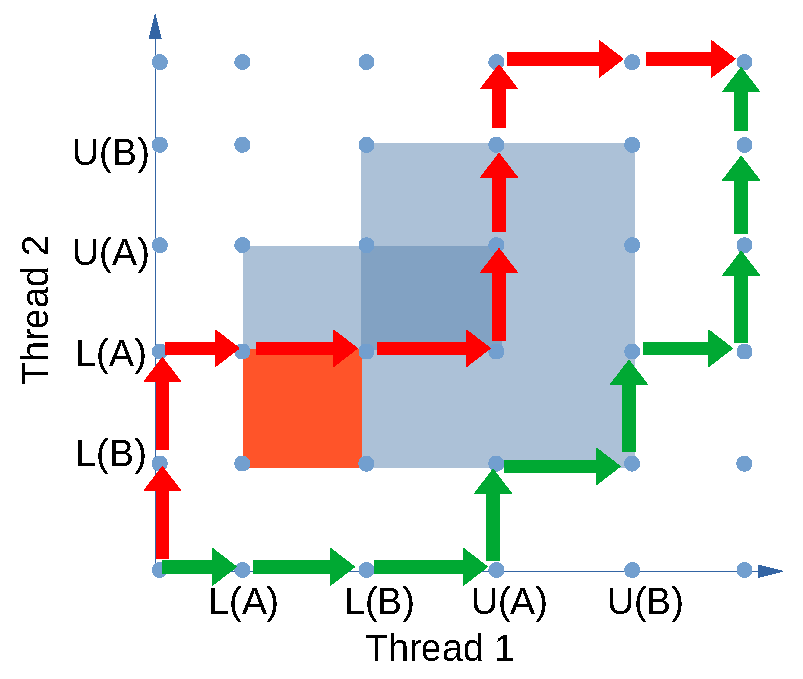
\includegraphics[width=\textwidth]{img/progress-deadlock.pdf}
  \caption{A progress graph of the two potentially deadlocking threads.}
  \label{fig:progress-deadlock}
\end{figure}

As each thread is sequential, its progress can be mapped by following along its axis, with any point in the graph being an expression of the combined states of both graphs. For example, the bottom left corner would be neither thread having started yet, with the top right corner being both threads having completed. The shaded blue section shows forbidden zones, where due to our mutexes is an impossible state to reach. There are two overlapping zones here, one for mutex A and one for mutex B, with them each overlapping in the middle of the graph. We can derive the locations of these zones by taking the coordinate of where each thread locks the mutex as the bottom left corner, and the coordinate of where each thread unlocks the mutex as the top right corner.

Two traces have been shown through the graph, one in green and one in red. The green shows a valid route through that does not enter any forbidden zone and so will produce a valid result. The red is an impossible trace as it enters a state within the forbidden zones, and so cannot occur in practice.

The concerning part of this graph is the red shaded area towards the bottom left of the graph. This shows a potential deadlock. As each thread can only progress linearly, our route through the graph can only be parallel to either axis. If our state ever enters the red zone then there is no way to escape as progress is blocked by the two forbidden zones. This makes it trivial to say that if we can draw a progress graph, if it none of these progress traps exist then our system is deadlock free. A solution to this is to reorder the operations our threads perform. This can be seen in figure \ref{fig:progress-safe} where both threads are now locking and unlocking the mutexes in the same order. No progress traps exist and any valid state has at least one path out of, therefore we are always deadlock free.

\begin{figure}
  \centering
  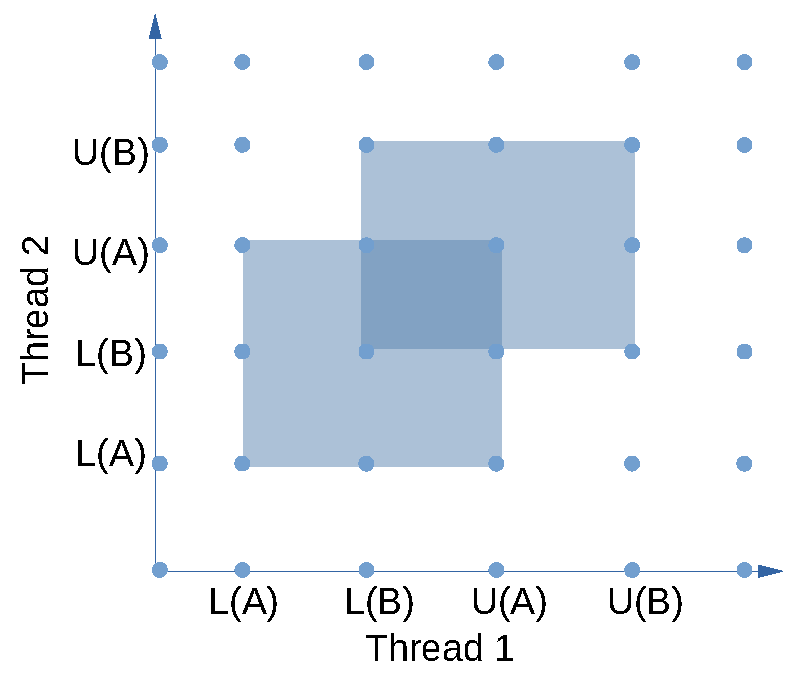
\includegraphics[width=\textwidth]{img/progress-safe.pdf}
  \caption{A progress graph of the two never deadlocking threads.}
  \label{fig:progress-safe}
\end{figure}

%%% Local Variables:
%%% mode: latex
%%% TeX-master: "notes"
%%% End:


\chapter{Parallel Speedup and Scalability}
\label{chap:scaling}

While \emph{concurrent programming} is often done to model the problem
domain nicely (e.g. have a thread per connection to a web server),
\emph{parallel programming} is primarily concerned with speeding up
our programs.  This chapter will introduce nomenclature for talking
about and comparing the performance of programs, and also discuss ways
in which we can predict the potential performance advantage from
parallelising a program.

\section{Speedup}
\label{sec:speedup}

Suppose we are given some program and asked to speed it up.  We then
hack on it for a bit based on our knowledge of low-level programming.
But how do we quantify our improvements?  The standard approach to
comparing the performance of two programs is by computing the
\emph{speedup} of one over the other.

\subsection{Speedup in latency}
\label{sec:speedup-in-latency}

The easiest way to quantify the performance of a program by itself is
to run it and measure how long it takes.  This is called program
\emph{latency} (often called \emph{runtime}): how long from it starts
until the result is ready?  This is usually measured in \emph{wall
  time}, because it corresponds to the real-world time we can measure
with a clock on our wall.  In contrast to this is \emph{CPU time},
which is the total amount of time spent executing code on the CPUs we
have available.  When we parallelise a program, we decrease the wall
time, but typically not the CPU time---$16$ CPUs that simultaneously
run for $60$ seconds equates $960$ seconds of total CPU time, but will
only have taken $60$ seconds of wall time.

We usually have to put in effort to make sure that our time
measurement is reliable.  For example, we must make sure that we are
measuring what we intend to measure---sometimes we do not wish to
measure e.g. startup overhead, or loading data from files.  It's also
an easy mistake to make to measure CPU time rather than wall time,
which will hide the advantage of parallelisation.  Also, particularly
with short-running programs, we must perform multiple measurements to
average out random timing effects caused by random scheduling
decisions taken by the operating system, or background tasks waking up
and causing cache evictions.  As a final concern, we must also make
sure that we are compiling with optimisations, for example by passing
\texttt{-O3} to the C compiler.  You may be used to passing
\texttt{-g}, which is good for debugging, but hinders the performance
of the generated code.

Once we have reliable runtime measurements for both the original
program and our modified program, we compare them by computing the
\emph{speedup}:

\begin{definition}[Speedup in latency]\label{speedup-latency}

  If $T_{1}, T_{2}$ are the runtimes of two programs $P_{1}, P_{2}$,
  then the \emph{speedup in latency} of $P_{2}$ over $P_{1}$ is
  \[
    \frac{T_{1}}{T_{2}}
  \]
\end{definition}

For example, if we have a sequential program that runs in $25s$ and we
manage to write a parallel program that runs in $10s$ on our machine,
then we compute the speedup of the parallel program as

\[
  \frac{25}{10} = 2.5
\]

We would then say that the speedup we obtain is $2.5$.  Speedup is a
dimensionless quantity, but it's common to write it with a tailing
$\times$, as in $2.5\times$.  The speedup formula can explain why
programmers sometimes say ``program A is twice as fast as B'', when
they really mean ``program A runs in half the time as B''---they are
talking about the speedup being $2$.

\subsection{Speedup in throughput}

Latency speedup is useful for programs where the workload is
\emph{fixed}.  But sometimes we are in a situation where the workload
is infinite, for example in a long-running server that constantly
processes new requests.  Here latency is only meaningful within a
single request, and to quantify the performance of the entire system,
it is more interesting to look at the \emph{throughput} of how many
requests per time unit can be processed.  Measuring throughput also
allows us to compare the performance of programs that operate on
different data sets.

The throughput $Q$ is computed simply as the \emph{workload} $W$
processed in some time-span $T$:

\[
  Q = \frac{W}{T}
\]

How we measure the workload depends on the concrete program.  For a
web server, we would measure requests.  For matrix multiplication, we
might measure total number of input elements accessed.  Once we have
computed throughput, we can then compute the speedup.

\begin{definition}[Speedup in throughput]\label{speedup-throughput}

  If $Q_{1}, Q_{2}$ are the throughputs of two programs
  $P_{1}, P_{2}$, then the \emph{speedup in throughput} of $P_{2}$
  over $P_{1}$ is
  \[
    \frac{Q_{2}}{Q_{1}}
  \]
\end{definition}

For example, suppose we have a program $P_{1}$ that can sum a megabyte
in $69\mu{}s$, and a program $P_{2}$ that can sum a gigabyte in
$28,589\mu{}s$.  Since the workloads are different, we cannot directly
compare their latency, but we can compute the throughputs as follows:

\begin{align*}
  Q_{1} =& \frac{2^{10}B}{69\mu{}s} = 15196 \textrm{B}/\mu{}\textrm{s} = 14.2 \textrm{GiB}/\textrm{s} \\
  Q_{2} =& \frac{2^{30}}{28589} = 37558 \textrm{B}/\mu{}\textrm{s} = 35.0 \textrm{GiB}/\textrm{s}
\end{align*}

The speedup in throughput of $P_{2}$ over $P_{1}$ is

\[
  \frac{35.0 \textrm{GiB}/\textrm{s}}{14.2 \textrm{GiB}/\textrm{s}} = 2.46
\]

Note that while lower numbers are better for latency, higher numbers
are better for throughput.  In both cases, a higher speedup is better.

\section{Scalability}

By \emph{scalability} we mean how the system improves in its capacity
(runtime or throughput) as we add more resources, such as more
processors.  It can also be used to describe how the performance
changes as the problem size increases---this is essentially what
big-$O$ notation is for.  With respect to parallelisation, we are
interested in how the performance of a system changes as we add or
exploit more processors.  We distinguish two forms of scalability.

\begin{definition}[Strong scaling]
  How the runtime varies with the number of processors for a fixed
  problem size.
\end{definition}

\begin{definition}[Weak scaling]
  How the runtime varies with the number of processors for a fixed
  problem size \textit{relative to the number of processors}.
\end{definition}

\subsection{Amdahl's Law}

Before we start on the often significant task of parallelising a
program, or using a larger and more parallel computer to run it, it is
worthwhile to estimate the potential performance gain.  Unfortunately,
it is not all parts of a program that benefit from increased
parallelisation.  For example, suppose a program needs 20 hours to
run, but a 1-hour part of the program cannot possibly be parallelised.
This is not unlikely: perhaps that hour is spent reading configuration
data, loading code, formatting human-readable reports, or waiting for
the human operator to interact with the system somehow.  Even if we
optimise the program such that the optimisable 95\% of the program
runs in \emph{zero time}, we have only achieved a speedup of $20$.

Gene Amdahl inspired the now-famous \emph{Amdahl's
  Law}~\cite{10.1145/1465482.1465560} to describe the theoretical
speedup from parallelisation:

\begin{definition}[Amdahl's Law]\label{amdahl}

  If $p$ is the proportion of execution time that benefits from
  parallelisation, then $S(N)$ is maximum theoretical speedup
  achievable by execution on $N$ threads, and is given by
  \[
    S(N) = \frac{1}{(1-p)+\frac{p}{N}}
  \]
\end{definition}

We can see that

\[
  S(N) \leq \frac{1}{1-p}
\]

This means that the potential speedup by optimising part of a system
is bounded by how dominant this part is in the overall runtime.  It
tells us that we should spend our time optimising the parts that take
the most time to run.  As \cref{fig:amdahl} shows, it is a rather
pessimistic law---even in the case where 99\% of the program can be
parallelised, execution on 300 processors will give us a speedup of
about $75$ over a single processor.

While Amdahl's Law is usually applied to parallelisation, it can be
used to characterise \emph{any} situation where we are optimising a
part of some system.

\begin{figure}
  \centering
  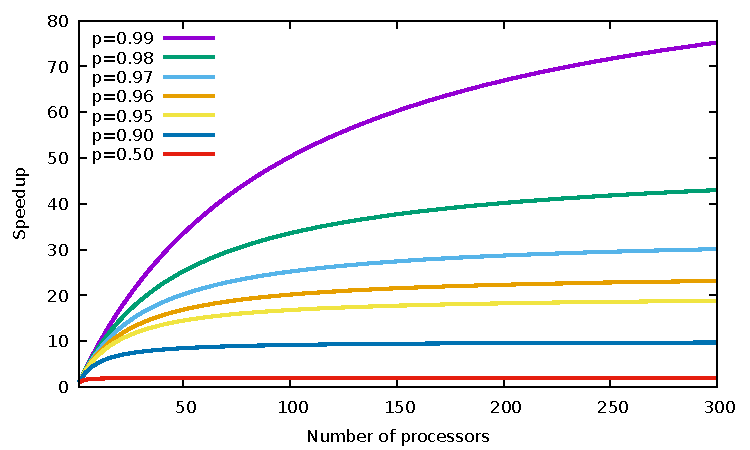
\includegraphics[width=\textwidth]{img/amdahl.pdf}
  \caption{A graph of Amdahl's Law, plotted for various values of $p$.}
  \label{fig:amdahl}
\end{figure}

\subsection{Gustafson's Law}
\label{sec:gustafson}

As parallel supercomputers became more common in the 80s, researchers
found that they routinely achieved speedup far in excess of what
Amdahl's Law would predict.  This is because Amdahl's Law is quite
pessimistic, as it assumes that the workload stays \emph{fixed} as we
gain access to more computational resources.  In practice, as
workloads increase in size, the parallelisable fraction tends to
\emph{increase} in its share of the overall runtime.  Also, when we
get access to a larger machine, we tend not to be interested in
solving our old problems faster, but in solving bigger problems in the
same time as it took to solve our old problems.  \emph{Time} is the
constant, not the workload.

Suppose we scale the runtime to be $1$ and use $s,p$ to indicate the
fraction of this unit runtime spent in sequential and parallel code
respectively on a parallel system with $N$ threads.  Then a sequential
processor would require $s+N\times{}p$ time to execute the program.
The scaled speedup of parallel execution is then

\begin{equation*}
  \frac{s+p\times N}{s+p} \\
  = s+p\times N \\
  = N + (1-N) \times s
\end{equation*}

This observation was first published by John
L. Gustafson~\cite{10.1145/42411.42415} and is therefore called
Gustafson's Law:

\begin{definition}[Gustafson's Law]\label{gustafson}
  If $s$ is the proportion of execution time that must be sequential,
  then $S(N)$ is maximum theoretical speedup achievable by execution
  on $N$ threads, and is given by

  \[
    S(N) = N + (1-N) \times s
  \]
\end{definition}

\begin{figure}
  \centering
  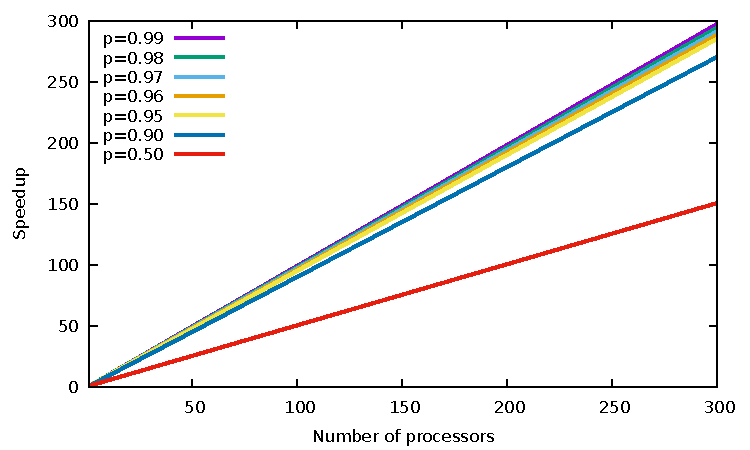
\includegraphics[width=\textwidth]{img/gustafson.pdf}
  \caption{A graph of Gustafson's Law, plotted for various values of
    $p$ (note that $p=1-s$).}
  \label{fig:gustafson}
\end{figure}

Compared to Amdahl, Gustafson is much more of an optimist---as shown
on \cref{fig:gustafson}, Gustafson's Law plots as a \textit{line},
meaning that the speedup as we add more processors is \textit{linear}.

Neither Amdahl's nor Gustafson's Laws are \emph{laws} in the common
sense of the word.  Despite providing conflicting predictions, they
can both be true under different circumstances.  Amdahl's Law tells us
about the limitations of parallelism under a fixed workload, while
Gustafson's Law tells us about the limitations of parallelism where we
assume we the workload grows proportionally with the amount of
parallelism.  Broadly, Amdahl's Law predicts strong scalability, and
Gustafson's law predicts weak scalability.

Both laws make significant simplifying assumptions---in practice,
little scientific code consists of enormous fully parallel loops with
completely independent iterations, but will tend to require some form
of routine communication, proportional to the number of processors
involved.  Specifically, these laws tend to discount the nonlinear
scaling of accessing large amounts data due to locality effects.

%%% Local Variables:
%%% mode: latex
%%% TeX-master: "notes"
%%% End:


\lstset{language=C}

\chapter{Loop Dependence Analysis}
\label{chap:dependencies}

\begin{quote}
  \emph{This chapter is adapted with permission from the PMPH Lecture
    Notes written by Cosmin Oancea.}
\end{quote}

So far, we have assumed that the user writes a fresh implementation of
a known algorithm, and that it can be straightforwardly expressed as
fully parallel loops, or as a simple reduction.  However, there is a
lot of legacy sequential scientific code written in imperative
languages such as C++, Java, Fortran, and either the precise algorithm
to which they correspond to (i) may have been forgotten (not
documented), or (ii) a fresh implementation is infeasible (e.g.,
because it costs too much).  At some point you may wish (or be asked)
to parallelise such code to run efficiently on a certain hardware.

This will require you to:

\begin{enumerate}
\item Identify the loop nests\footnote{A \emph{loop nest} is a
    collection of multiple loops nested within each other.} where most
  of the runtime is spent.

\item Parallelise these loops by reasoning at a low level of
  abstraction about which loops in the nest are parallel.

\item Decide on the manner in which loop nests can be re-written in
  order to optimise locality of reference, load balancing, thread
  divergence, etc.
\end{enumerate}

The main source of inspiration for the material presented in this and
\cref{chap:loop-transformations} has been the book ``Optimizing
compilers for modern architectures: a dependence-based
approach''~\cite{kennedy2001optimizing}.

This chapter is organised as follows:
\begin{itemize}
\item \Cref{sec:dir-vct} introduces various nomenclature,
  in particular the notion of cross-iteration dependency, and
  it shows how to summarise dependencies across the iteration
  space into a succinct representation, named direction vectors,
  that promotes reasoning about various code transformations.
\item \Cref{sec:loop-par} presents a simple theorem that allows easy
  identification of loop-level parallelism.
\end{itemize}

\section{Direction vectors}
\label{sec:dir-vct}

We start by defining the various reasons why a program statement must
be executed after some previous.  C executes statements in
\emph{program order}---the order they occur in the source code.
Dependence analysis is about distinguishing when the program order is
crucial for correct execution, and in which cases it is arbitrary
because C requires us to write statements in \emph{some} order.  If a
statement $S_{2}$ \emph{depends} on $S_{1}$, then $S_{2}$
must always be executed after $S_{1}$.  Dependencies typically
arise because the two statements interact with the same values, with
at least one of the statements changing the value.  When two
statements are not dependent on each other, they can in principle be
executed in parallel.  Our goal is to use dependence analysis to
identify when entire \emph{loop iterations} are independent, which
means that they can be executed in parallel.

\begin{figure}
  \centering
  \begin{subfigure}[t]{0.32\textwidth}
\begin{lstlisting}
S1:   X  = ..
S2:   .. = X
\end{lstlisting}
\caption{RAW: Read after write.}
\label{fig:raw}
  \end{subfigure}
  \hfill
  \begin{subfigure}[t]{0.32\textwidth}
\begin{lstlisting}
S1:   .. = X
S2:   X  = ..
\end{lstlisting}
\caption{WAR: Write after read.}
\label{fig:war}
  \end{subfigure}
  \hfill
  \begin{subfigure}[t]{0.33\textwidth}
\begin{lstlisting}
S1:   X = ...
S2:   X = ...
\end{lstlisting}
\caption{WAW: Write after write.}
\label{fig:waw}
  \end{subfigure}
  \caption{Three different kinds of dependencies.}
  \label{fig:dependencies}
\end{figure}

The possible kinds of dependencies are depicted in
\cref{fig:dependencies} between two statements $S_{1}$ and
$S_{2}$, which reside for simplicity in the same \emph{basic
  block}---a straight-line of code which is always entered by the
first statement and is exited after the execution of the last
statement.  For example, the body of a loop can be considered a basic
block if it contains no control flow and no
\texttt{continue}\\texttt{break} statements.  The possible kinds of
dependencies are as follows:

\begin{description}
\item[RAW (\cref{fig:raw}):] refers to the case when a write to a
  register or memory location is followed, in program order, by a read
  from the same register or memory location; this is typically
  referred to as a read-after-write hazard in hardware-architecture
  nomenclature, and as a \emph{true} dependency in loop-based analysis
  nomenclature. The word \emph{true} refers to the fact that such a
  dependency denotes a producer-consumer relation, in which the value
  produced by $S_{1}$ is used in $S_{2}$. The
  producer-consumer relation is an algorithmic property of the
  program; such a dependency cannot be eliminated other than by
  changing the underlying algorithm.

\item[WAR (\cref{fig:war}):] refers to the case when a read from a
  register or memory location is followed, in program order, by a
  write to the same register or memory location; this is referred to
  as a write-after-read hazard, and equivalently as an \emph{anti}
  dependency. The problem here is that, if the two statements are
  reordered---meaning $S_{2}$ executes before $S_{1}$, then
  the value needed by $S_{1}$ is no longer available because it
  has been already overwritten by $S_{2}$.

\item[WAW (\cref{fig:waw}):] refers to the case when a write from a
  register or memory location is followed, in program order, by
  another write to the same register or memory location; this is
  referred to as a write-after-write hazard, and equivalently as an
  \emph{output} dependency. The problem here is that, if the two
  statements are reordered---meaning $S_{2}$ executes before
  $S_{1}$, then the final value stored in register or memory
  location is that of $S_{1}$ rather than that of $S_{2}$.
\end{description}

In what parallelism or loop analysis is concerned, we are primarily
interested in analysing the (true, anti and output) \emph{dependencies
  that occur across different iterations of the loop}. For example such
a true dependency would correspond to the case in which an early
iterations \texttt{i} writes/produces an array element that is
subsequently read/consumed in a later iteration \texttt{j > i}.

In what parallelisation is concerned, the main limiting factor are the
true dependencies---which correspond to an algorithmic
property---because the anti and output dependencies can be typically
eliminated by various techniques, as we shall see.

\subsection{Loop notation and lexicographic ordering of iterations in a loop nest}

In the following we are concerned with loop nests that consist of
\lstinline{for}-loops where the number of iterations (the \emph{trip
  count}) can be determined when the loop is first entered.  This is
the case when:
\begin{enumerate}
\item The loop counter is not modified inside the loop.
\item The loop condition is of the form $i < n$, where $i$ is the loop
  counter and $n$ does not change during execution of the loop.
\item The loop counter is increased by a constant for each loop
  iteration.
\end{enumerate}
Most \lstinline{for}-loops you have written probably satisfy these
conditions.

In the following we will also assume that iterations in a loop
nest are represented by a vector, in which iterations numbers
are written down from the corresponding outermost to the innermost
loop in the nest, and are ordered \emph{lexicographically}---i.e.,
are ordered consistently with the order in which they are executed
in the (sequential) program. This means that in the loop nest below:
\begin{lstlisting}[mathescape=true]
for (int i = 0; i < N; i++)
  for (int j = 0; j < M; j++)
    ... loop-nest body ...
\end{lstlisting}
iteration \texttt{$\vec{k}$=(i=2,j=4)} is smaller than iteration
\texttt{$\vec{l}$=(i=3,j=3)} (i.e., $\vec{k} < \vec{l}$), because the
second iteration of the outer loop is executed before the third
iteration of the outer loop, no matter what the iteration numbers are
executed for the inner loop (of index \texttt{j}).  In essence the
iteration numbers of inner loops are only used to discriminate the
order in the cases in which all the outer-loop iterations are equal,
for example \texttt{$\vec{k}$=(i=3,j=3) $<$
  $\vec{l}$=(i=3,j=4)}

\subsection{Dependency definition}
The precise definition of a dependency between two statements
located inside a loop nest is given below.

\begin{definition}[Loop Dependency]\label{Loop-Dep}
  There is a dependency from statement $S_1$ to statement $S_2$
  in a loop nest {\em if and only if} there exists loop-nest
  iterations $\vec{k}$, $\vec{l}$ such that $\vec{k} \leq \vec{l}$
  and there exists an execution path from statement $S_{1}$ to
  statement $S_{2}$ \emph{such that:}
  \begin{description}
  \item[1.] $S_{1}$ accesses some memory location $M$ in iteration $\vec{k}$, and
  \item[2.] $S_{2}$ accesses the same memory location $M$ in iteration $\vec{l}$, and
  \item[3.] one of these accesses is a write.
  \end{description}
  In such a case, we say that $S_1$ is the \emph{source} of the dependence,
  and that $S_{2}$ is the \emph{sink} of the dependence, because $S_1$ is supposed
  to execute before $S_2$ in the sequential program execution.\\
  Dependencies can be visually depicted by arrows pointing from the source
  to the sink of the dependence.
\end{definition}

The definition basically says that in order for a dependency to exist,
there must be two statements that access \emph{the same memory
  location} and one of the accesses must be a write---two read
instructions to the same memory location do not cause a
dependency. The nomenclature denotes the statement that executes first
in the program order as \emph{the source} and the other as \emph{the
  sink} of the dependency. We represent a dependency graphically with
an arrow pointing from the source to the sink.

Optimisations for instruction-level parallelism (ILP)---meaning
eliminating as much as possible the stalls from processor's pipeline
execution\footnote{Outside the scope of HPPS.}---typically rely on
intra-iteration analyses (i.e., $\vec{k}=\vec{l}$).  Higher-level
optimisations, such as detection of loop parallelism, are mostly
concerned with analysing inter-iteration dependencies (i.e.,
$\vec{k}\neq\vec{l}$).  For example the main aim could be to disprove
the existence of inter-iteration dependencies, such that different
iterations may be scheduled out of order (in parallel) on different
cores, while the body of an iteration is executed sequentially on the
same core. In such a context, intra-iteration dependencies are
trivially satisfied, and so are not very interesting.

\subsection{Aggregating dependencies with direction vectors}

Assume the three loops presented in \cref{fig:data-dep-running-eg},
which will be used as running example to demonstrate data dependence
analysis and related transformations. We make the important
observation that the code is not in three-address code (TAC) form: a
statement such as \texttt{A[j][i] = A[j][i] + 3} would correspond to
three TAC or hardware instructions: one that loads from memory
\texttt{tmp1 = A[j][i]}, followed by one that performs the arithmetic
operation \texttt{tmp2 = tmp1 + 3}, followed by one that writes to
memory \texttt{A[j][i] = tmp2}. Automated analysis is for simplicity
usually carried out on programs in TAC form but, for brevity, our
analysis will be carried out at the statement level.
% ---however please remember that such a statement
% is actually a composition of three hardware instructions!
A human may start analysing dependencies:
\begin{itemize}
\item by depicting the iteration space in a rectangle in which the $x$
  axis and $y$ axis correspond to iteration numbers of the inner
  loop $j$ and outer loop $i$, respectively, and
\item then by reasoning point-wise about what dependencies may
  happen between two iterations.
\end{itemize}

\begin{figure}
  \centering

  \begin{subfigure}[b]{0.45\textwidth}
\begin{lstlisting}[language=C,mathescape=True]
for (int i = 0; i < N; i++)
  for (int j = 0; j < N; j++)
    $S_1:$ A[j][i] = A[j][i]...
\end{lstlisting}
    \caption{}
    \label{fig:data-dep-running-eg-a}
  \end{subfigure}

  \begin{subfigure}[b]{0.45\textwidth}
\begin{lstlisting}[language=C,mathescape=True]
for (int i = 1; i < N; i++)
  for (int j = 1; j < N; j++) {
    $S_1:$ A[j][i] = A[j-1][i-1]...
    $S_2:$ B[j][i] = B[j-1][i]...
  }
\end{lstlisting}
    \caption{}
    \label{fig:data-dep-running-eg-b}
  \end{subfigure}

  \begin{subfigure}[b]{0.45\textwidth}
\begin{lstlisting}[language=C,mathescape=True]
for (int i = 1; i < N; i++)
  for (int j = 0; j < N; j++)
    $S_1:$ A[i][j] = A[i-1][j+1]...
\end{lstlisting}
    \caption{}
    \label{fig:data-dep-running-eg-c}
  \end{subfigure}

  \caption{Three simple running code examples that will be used to
    demonstrate data-dependency analysis and related transformation.
    Note that the statement labels $S_{i}$ are not part of the code as
    such, but used to refer to specific statements in the text.}
  \label{fig:data-dep-running-eg}
\end{figure}

\begin{figure}
  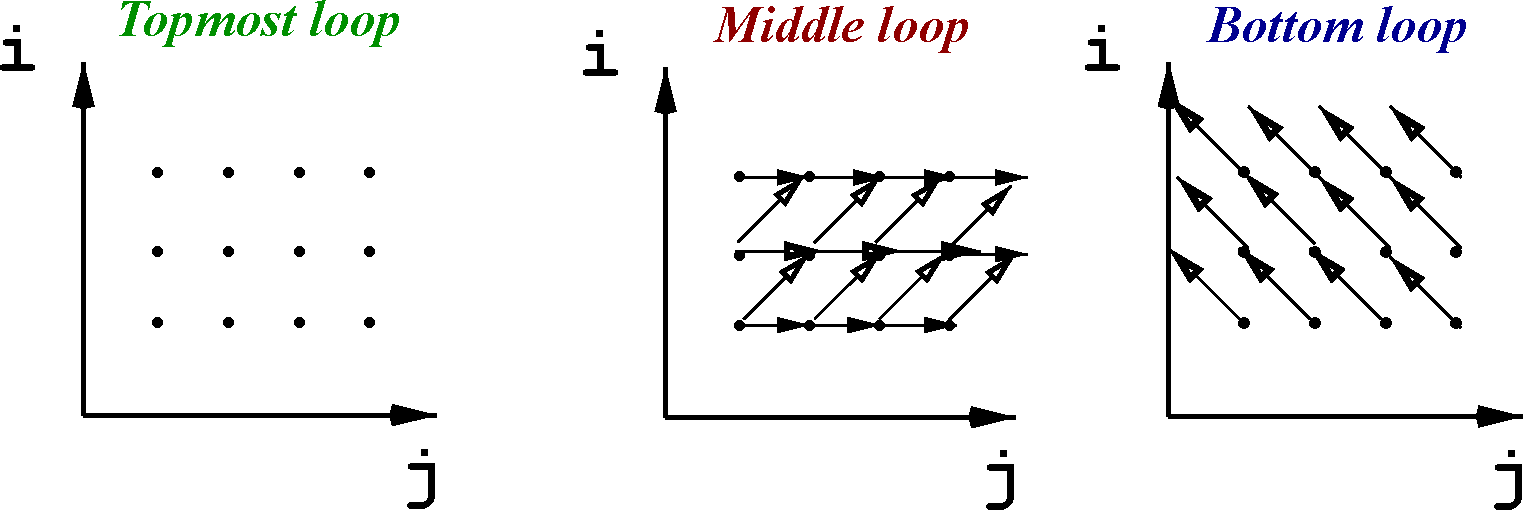
\includegraphics[width=\textwidth]{img/LoopDeps.pdf}
  \caption{Graphical representation of the dependencies for the three running examples shown in \cref{fig:data-dep-running-eg}; the $x$ and $y$ axis correspond to the index of the inner and outer \lstinline{do} loop, respectively.}
  \label{fig:dep-graph}
\end{figure}

A graphical representation of the dependencies of the three running code
examples is shown in \cref{fig:dep-graph}.   They can be intuitively inferred
as follows:
\begin{itemize}
\item For the loop in \cref{fig:data-dep-running-eg-a}, different
  loop-nest iterations $(i_1,j_1)$ and $(i_2,j_2)$ necessarily read
  and write different array elements \texttt{A[$j_1$][$i_1$]} and
  \texttt{A[$j_2$][$i_2$]}.  This is because our assumption is that
  $(i_1,j_1) \neq (i_2,j_2)$, hence it cannot be that both $i_1 = i_2$
  and $j_1 = j_2$. As such, the representation of dependencies should
  be a set of points (no arrows), meaning that all dependencies
  actually occur inside the same iteration---in fact they are anti
  intra-iteration dependencies (WAR) because \texttt{A[j][i]} is read
  first and then \texttt{A[j][i]} is written inside the same
  iteration.
\item For the loop in \cref{fig:data-dep-running-eg-b} we reason
  individually for statements $S_1$ and $S_2$ because each statement
  accesses (one) array \texttt{A} and \texttt{B}, respectively:
  \begin{itemize}
  \item[$S_1:$] Let's take an iteration, say $(i_1=2, j_1=3)$,
    which \emph{reads} element \texttt{A[$j_1$-1][$i_1$-1] = A[2][1]}.
    Since an iteration $(i,j)$ always writes the element
    \texttt{A[i][j]}, we can reason that iteration $(i_2=1, j_2=2)$
    will \emph{write} the same element \texttt{A[2][1]}.
    It follows that we have discovered a true (RAW) dependency,
    depicted in the figure with and arrow, from the source
    iteration $(i_2=1, j_2=2)$---which writes \texttt{A[2][1]}---to
    the sink iteration $(i_1=2, j_1=3)$---which reads \texttt{A[2][1]}.
    This is because iteration $(1,2) < (2,3)$ according to the
    lexicographical ordering, and as such, the read happens after
    the write (RAW) in program order. One can individually reason
    for each point of the iteration space and fill it with oblique,
    forward-pointing arrows denoting true dependencies between
    different instances of statement $S_1$
    (executing in different iterations).
  \item[$S_2:$] Following a similar rationale, iteration $(i_1=2, j_1=3)$
    \emph{reads} element \texttt{B[$j_1$-1][$i_1$] = B[2][2]}, and
    iteration $(i_2=2, j_2=2)$ \emph{writes} element \texttt{B[2][2]}.
    It follows that we have discovered a true (RAW) dependency
    with source $(i_2=2, j_2=2)$ and sink $(i_1=2, j_1=3)$,
    because $(2,2) < (2,3)$ in lexicographic ordering.
    Since $i_1=i_2$ we depict the arrow parallel with the
    horizontal axis (that depicts values of $j$). One can
    fill in the rest of the iteration space with horizontal arrows.
  \end{itemize}

\item For the loop in \cref{fig:data-dep-running-eg-c} we reason in a
  similar way: take iteration $(i_1=2, j_1=3)$ that \emph{reads}
  element \texttt{A[2-1][3+1] = A[1][4]}. This element is
  \emph{written} by iteration $(i_2=1,j_2=4)$. It follows that we have
  discovered a true (RAW) from source $(i_2=1,j_2=4)$ to sink
  $(i_1=2, j_1=3)$---because the read happens in iteration $(2,3)$
  which comes after the write in iteration $(1,4)$, i.e.,
  $(1,4) < (2,3)$.  Thus, one can fill in the iteration space with
  oblique, backward-pointing arrows, denoting true dependencies
  between instances of $S_1$ executing in different iterations.
\end{itemize}

We have applied above a human type of reasoning and, as a result, we
have a graphical representation of all dependencies. However, such a
reasoning is not suitable for automation because (i) the loop counts
are statically unknown---they depend on the dataset---hence one cannot
possibly represent an arbitrary large iteration space, and, more
importantly, (ii) even if the loop counts would be statically known it
is still inefficient to maintain and work with all this pointwise
information.

A representation that promotes automated reasoning should succinctly
capture the repeated pattern in the figure. Intuitively and
imprecisely, for \cref{fig:data-dep-running-eg-a} the pattern would
correspond to a point, for \cref{fig:data-dep-running-eg-b} it would
correspond to two arrows---one oblique and one horizontal forward
pointing arrows---and for \cref{fig:data-dep-running-eg-c} it would
correspond to an oblique, backward-pointing arrow.
%
These patterns are formalized by introducing the notion of
\emph{direction vectors}.

\begin{definition}[Dependency direction vector]\label{Dep-Dir-Vect}

  Assume there exists a dependency with source $S_{1}$ in iteration $\vec{k}$
  to sink $S_{2}$ in iteration $\vec{l}$ ($\vec{k}\leq\vec{l}$).
  We denote by $m$ the depth of the loop nest, we use $i$ to range
  from $0,\ldots,m-1$, and we denote by $x_i$ the $i^{th}$
  element of some vector $\vec{x}$ of length $m$.

  The \emph{direction vector} between the instance of statement $S_1$
  executed in some source iteration $\vec{k}$ and statement $S_2$
  executed in sink iteration $\vec{l}$ is denoted by
  $\vec{D}(S_1\in\vec{k},S_{2}\in\vec{l})$, and corresponds to a vector
  of length $m$, whose elements are defined as:

  \begin{equation}
    D_i(S_1\in\vec{k},S_2\in\vec{l})=
    \begin{cases}
      \mbox{\texttt{<}} \ \ \ \ \mbox{\textrm{if it is provably that}} ~~k_i ~<~ l_i,\\
      \mbox{\texttt{=}} \ \ \ \ \mbox{\textrm{if it is provably that}} ~~k_i ~=~ l_i,\\
      \mbox{\texttt{>}} \ \ \ \ \mbox{\textrm{if it is provably that}} ~~k_i ~>~ l_i,\\
      \mbox{\texttt{{}*}} \ \ \ \ \mbox{\textrm{if}}~k_i ~\mbox{\textrm{{}and}}~ l_i~\mbox{are statically uncomparable.}\\
    \end{cases}
    \label{eqn:dir-vec}
 \end{equation}
\end{definition}

The first three cases of the definition above assume that the ordering
relation between $k_i$ and $l_i$ can be statically derived in a generic
fashion (for any source $k_i$ and $l_i$); if this is not possible than
we use the notation \texttt{*} which \emph{conservatively} assumes that any
directions may be possible---i.e., star should be understood as
simultaneous existence of all \texttt{<, =, >} directions. For example,
the loop
\begin{lstlisting}[mathescape=true]
for (int i = 0; i < N; i++)
  $S_1:$  A[ X[i] ] = ...
\end{lstlisting}
would result in direction vector \texttt{[*]} corresponding to a
potential output dependency (WAW), because the write access to
\texttt{A[ X[i] ]} is statically unanalysable---for example under the
assumption that the index array \texttt{X} is part of the
dataset---and, as such, all direction vectors may possibly hold
between various pairs of instances of statement $S_1$ executed in
different iterations.

Note that the symbols \texttt{<, =, >} are \emph{not} connected at all
to the type of the dependency, e.g., true (RAW) or anti (WAR)
dependency.  The type of the dependency is solely determined by the
operation of the source and that of the sink: If the source is a write
statement and the sink is a read then we have a true (RAW) dependency;
if the source is a read and the sink is a write then we have an anti
(WAR) dependency; if both source and sink are writes then we have an
output (WAW) dependency.

The meaning of the symbol \texttt{>} at some position $i$ is that
the source iteration at loop-level $i$ is greater than the sink
iteration at loop-level $i$. This case is possible, for example
the code in \cref{fig:data-dep-running-eg}(c) shows a dependency
with source iteration $(1,4)$ and sink iteration $(2,3)$. At the
level of the second loop, we have $4 > 3$ hence the direction
is \texttt{>} but still the source iteration is less than the sink
iteration $(1,4) < (2,3)$ because of the first loop level.
This observation leads to the following corollary:

\begin{corollary}[Direction vector legality]\label{Leg-Dir-Vect}

  A direction vector is legal (well formed), if removing the
  \texttt{=} entries does \emph{not} result in a leading \texttt{>}
  symbol, as this would mean that an iteration depends on a future
  iteration, and depending on a future event is considered impossible,
  and as such illegal.
\end{corollary}

It remains to determine the sort of reasoning that can be applied to
compute the direction vectors for the code examples in
\cref{fig:data-dep-running-eg}:
\begin{description}
\item[The loop in \cref{fig:data-dep-running-eg-a}:] dependencies can
  occur only between instances of statement $S_1$, executed in
  different (or the same) iterations.  We recall that, by the
  definition of dependency, the two (dependent) iterations must access
  the same element of \texttt{A} and at least one iteration should
  perform a write.  Since statement $S_1$ performs a read and a write
  to elements of array \texttt{A}, two kinds of dependencies may
  occur:
  \begin{description}
  \item[WAW:] an output dependency may be caused by two write accesses
    in two different iterations, denoted $(i_1,j_1)$ and
    $(i_2,j_2)$. The written element is thus \texttt{A[j$_1$][i$_1$]},
    which must be the same as \texttt{A[j$_2$][i$_2$]} for a
    dependency to exist. By \cref{eqn:dir-vec} this results in the
    system of equations
    \[
      \begin{cases}i_1 = i_2\\j_1 = j_2\end{cases}
    \]
    which leads to direction vector \texttt{[=,=]}.  Hence, an output
    dependency from $S_1$ to $S_1$ happens in the same iteration, but
    statement $S_1$ executes only one write access in the same
    iteration.  The conclusion is that no output dependency can occur,
    hence the direction vector is discarded.
  \item[RAW:] a true or anti dependency---we do not know yet
    which---will be caused by the read access from \texttt{A} and the
    write access to \texttt{A} in different (or same)
    iterations. Remember that a statement such as \texttt{A[j][i] =
      A[j][i] + 3} actually corresponds to three hardware
    instructions, hence either a cross- or an intra-iteration
    dependency will necessarily occur.  Assume some iteration
    $(i_1, j_1)$ reads from \texttt{A[j$_1$][i$_1$]} and iteration
    $(i_2,j_2)$ writes to \texttt{A[j$_2$][i$_2$]}.  In order for a
    dependency to exist, the memory location of the read and write
    must coincide; this results in the system of equations
    \[
      \begin{cases}i_1 = i_2\\j_1 = j_2\end{cases}
    \]
    from which we can derive the direction vector:
    \texttt{[=,=]}. This implies that the dependency happens in the
    same iteration, hence it is an intra-iteration dependency.
    Furthermore, since the write follows the read in the instruction
    order of an iteration, this is an anti dependency (WAR).
  \end{description}

\item[For the loop in \cref{fig:data-dep-running-eg-b}:] dependencies
  may possibly occur between instances of statement $S_1$
  and between instances of statement $S_2$. The case of
  output dependencies is disproved by a treatment similar
  to the bullet above. It remains to examine the dependency
  caused by a read and a write in different instances of
  $S_1$ and $S_2$, respectively:
  \begin{description}
  \item[$S_1$:] assume iteration $(i_1,j_1)$ and iteration $(i_2,j_2)$
    reads from and writes to the same element of \texttt{A},
    respectively. Putting this in \cref{eqn:dir-vec} results in the
    system
    \[
      \begin{cases}i_1-1 = i_2\\j_1-1 = j_2\end{cases}
    \]
    which necessarily means that $i_1 > i_2$ and $j_1 > j_2$.
    However, we do not know yet which iteration is the source and
    which is the sink. Assuming that $(i_1, j_1)$ is the source
    results in the direction vector \texttt{[>,>]}, which is illegal
    by \cref{Leg-Dir-Vect}, because a direction vector cannot start
    with the \texttt{>} symbol. It follows that our assumption was
    wrong: $(i_2, j_2)$ is the source and $(i_1, j_1)$ is the sink,
    which means that this is a cross-iteration true dependency
    (RAW)---because the sink iteration reads the element that was
    previously written by the source iteration---and its direction
    vector is \texttt{[<,<]}.
  \item[$S_2$:] a similar rationale can be applied to
    determine that two instances of $S_2$ generate
    a true cross-iteration dependency (RAW), whose
    direction vector is \texttt{[=,<]}. In short, using the
    same notation results in the system of equations
    \[
      \begin{cases}i_1 = i_2\\j_1-1 = j_2\end{cases}
    \]
    hence the source must be $(i_2,j_2)$ and the sink must be
    $(i_1,j_1)$ and the direction vector is \texttt{[=,<]}.
  \end{description}

\item[For the loop in \cref{fig:data-dep-running-eg-c}:] dependencies
  may possibly occur between instances of statement $S_1$.  Assume
  iteration $(i_1,j_1)$ and $(i_2,j_2)$ reads from and writes to the
  same element of \texttt{A}, respectively.  Putting this into
  \cref{eqn:dir-vec} results in the system
  \[
    \begin{cases}i_1-1 = i_2\\j_1+1 = j_2\end{cases}
  \]
  which necessarily implies that $i_1 > i_2$ and $j_1 < j_2$. Choosing
  $(i_1,j_1)$ as the source of the dependency results in direction
  vector \texttt{[>,<]}, which is illegal because it has \texttt{>} as
  the first non-\texttt{=} outermost symbol, as stated by
  \cref{Leg-Dir-Vect}. It follows that $(i_1,j_1)$ must be the sink
  and $(i_2,j_2)$ must be the source, which results in the direction
  vector \texttt{[<,>]}, which is legal. Since the source writes and
  the sink reads, we have a true dependency (RAW).  Moreover since the
  direction vector indicates that the source iteration is strictly
  less than the sink iteration, this is also a cross-iteration
  dependency.
\end{description}

\begin{definition}[Dependency direction matrix]\label{Dep-Dir-Mat}
  A direction matrix is obtained by stacking together the
  direction vectors of all the intra- and cross-iteration
  dependencies of a loop nest (i.e., between any possible
  pair of write-write or read-read instruction instances).
\end{definition}

In conclusion, the direction matrices for the three running code
examples:

\begin{description}
\item[\Cref{fig:data-dep-running-eg-a}:]
  $\begin{cases}\texttt{[=,=]}\end{cases}$
\item[\Cref{fig:data-dep-running-eg-b}:]
  $\begin{cases}\texttt{[<,<]}\\\texttt{[=,<]}\end{cases}$
\item[\Cref{fig:data-dep-running-eg-c}:]
  $\begin{cases}\texttt{[<,>]}\end{cases}$
\end{description}

The following sections will show how the legality of powerful code
transformations can be reasoned in a simple way in terms of direction
vectors/matrices.

\section{Determining loop parallelism}
\label{sec:loop-par}

A loop is said to be parallel if its execution does not cause any
(true, anti, or output) dependencies between iterations---the loop
execution is assumed to be fixed in a specific iteration of an
(potentially empty) enclosing loop context.

The following theorem states that a sufficient condition for a loop to
be parallel is that for all the elements in the loop's corresponding
direction-matrix column, it holds that the element is either
\texttt{=} or there exists an outer loop whose corresponding direction
is \texttt{<} (on that row).  In the latter case we say that the outer
loop \emph{carries} all the dependencies of the inner loop, i.e.,
fixing an iteration of the outer loop (think executing the outer loop
sequentially) would guarantee the absence of cross-iteration
dependencies in the inner loop.

\begin{theorem}[Parallel loop]\label{Loop-Par}

  We assume a loop nest denoted by $\vec{L}$, whose direction matrix
  is denoted by $M$ and consists of $m$ rows.  A sufficient condition
  for a loop at depth $k$ in $\vec{L}$, denoted $L_k$, to be parallel
  is that $\forall i\in\{0,\ldots m-1\}~$ either $M[i][k]$ is
  \texttt{=} or there exists an outer loop at depth $q<k$ such that
  $M[i][q]$ is \texttt{<}.  Proof left as an exercise.
\end{theorem}

\Cref{Loop-Par} claims to give only a sufficient condition for loop
parallelism because it assumes that symbols such as \texttt{*} may be
part of the direction vector elements---we recall that \texttt{*}
conservatively assumes that all directions \texttt{<,=,>} may be
possible. If \texttt{*} does not appear in the direction matrix, then
the condition becomes \emph{necessary} as well as sufficient.  Let us
analyse the parallelism of each loop in our running examples:

\begin{description}
\item[\Cref{fig:data-dep-running-eg-a}:] The direction matrix is
  \texttt{[=,=]}, hence by \cref{Loop-Par}, both loops in the nest are
  parallel because all the directions are \texttt{=}.

\item[\Cref{fig:data-dep-running-eg-b}:] The direction matrix is
  \[
    M = \begin{cases}\texttt{[<,<]}\\\texttt{[=,<]}\end{cases}
  \]
  hence neither the outer nor the inner loop can be proven parallel by
  \cref{Loop-Par}. In the former case this is because $M[0,0]$ is
  \texttt{<} and there is no other outer loop to carry
  dependencies. In the latter case this is because $M[1,1]$ is
  \texttt{<} and the outer loop for that row has direction \texttt{=}
  (instead of \texttt{<}, which would have been necessary to carry the
  dependencies of the inner loop).

\item[\Cref{fig:data-dep-running-eg-c}:] The direction matrix is
  \texttt{[<,>]}, which means that the outer loop is not
  parallel---because it has a leading \texttt{<} direction---\emph{but
    the inner loop is parallel} because the outer loop starts with
  \texttt{<} on the only row of the direction matrix, and, as such, it
  carries all the dependencies of the inner loop.  To understand what
  this means, take a look again at the actual code in
  \cref{fig:data-dep-running-eg-c}.  Suppose we fix the outer
  iteration number to some value $i$. Then the read accesses always
  refer to row $i-1$ of matrix \texttt{A} and the write accesses
  always refer to row $i$ of \texttt{A}; hence a cross-iteration
  dependency cannot happen in the inner loop because no matter the
  value of $j$, the read and write statement instances cannot possibly
  refer to the same location of \texttt{A}.
\end{description}

%%% Local Variables:
%%% mode: latex
%%% TeX-master: "notes"
%%% End:


\lstset{language=C}

\chapter{Loop Transformations}
\label{chap:loop-transformations}

\begin{quote}
  \emph{This chapter is adapted with permission from the PMPH Lecture
    Notes written by Cosmin Oancea.}
\end{quote}

This chapter is organised as follows:
\begin{itemize}
\item \Cref{sec:loop-interch} presents a simple theorem that gives
  necessary conditions for the safety of the transformation that
  interchanges two perfectly nested loops.
\item \Cref{sec:loop-distrib} discusses the legality and
  the manner in which a loop can be distributed across the
  statements in its body.
\item \Cref{sec:false-dep-elim} discusses techniques for
  eliminating cross-iteration write-after-read and
  write-after-write dependencies.
\item \Cref{sec:strip-tiling} introducing a simple
  transformation, named stripmining, which is always valid, and
  shows how block and register tiling can be derived as a
  combination of stripmining, loop interchange and loop
  distribution.
\end{itemize}

\section{Loop interchange: legality and applications}
\label{sec:loop-interch}

Direction vectors are not used only for proving the parallel nature of
loops, but can also enable powerful code restructuring techniques. For
example they can be straightforwardly applied to determine whether it
is safe to interchange two loops in a perfect loop nest\footnote{ A
  perfect loop nest is a nest in which any two loops at consecutive
  depth levels are not separated by any other statements; for example
  all loop nests in \cref{fig:data-dep-running-eg} are perfectly
  nested.  }---which may result in better locality and even in
changing an inner loop nature from dependent (sequential) to
independent (parallel).

The following theorem gives a sufficient condition for the
legality of loop interchange---i.e., for the transformation
to result in code that is semantically equivalent to the original one.

\begin{theorem}[Legality of Loop Interchange]\label{Loop-Interch}
  A sufficient condition for the legality of interchanging two loops
  at depth levels $k$ and $l$ in a perfect nest is that interchanging
  columns $k$ and $l$ in the direction matrix of the loop nest
  \emph{does not result} in a (leading) \texttt{>} direction as the
  leftmost non-\texttt{=} direction of any row.
\end{theorem}

The theorem above shows that the legality of loop interchange
can be determined solely by inspecting the result of permuting
the direction matrix in the same way as the one desired for loops.
For the rationale related to why a row-leading \texttt{>} direction
is illegal, we refer the reader to \cref{Leg-Dir-Vect}: a non-\texttt{=}
leading \texttt{>} direction would correspond to depending on something
that happens in the future: this currently seems impossible in our
universe, and as such it signals an illegal transformation.
%
The following corollary can be easily derived from \cref{Loop-Interch}:

\begin{corollary}[Interchanging a parallel loop inwards]\label{Par-Loop-Interch}
  In a perfect loop nest, it is always safe to interchange a
  {\em parallel loop} inwards one step at a time (i.e., if the
  parallel loop is the $k^{th}$ loop in the nest then one can
  always interchange it with loop $k+1$, then with loop $k+2$, etc.).
\end{corollary}

The corollary says that if we somehow know the parallel nature
of a loop, then we can safely interchange it in the immediate inward
position, without even having to build the dependence-direction matrix.

Let us analyse the legality of loop interchange for the three loop
nests of our running example:

\begin{description}
\item[\Cref{fig:data-dep-running-eg-a}:] The direction matrix is
  \texttt{[=,=]} and, as such, it is legal to interchange the two
  loops, because it would result in direction matrix
  \texttt{[=,=]}. Moreover applying loop interchange in this case is
  highly beneficial because it \emph{optimises locality of reference}:
  the loop of index \texttt{i} appears in the innermost position after
  the interchange, which optimally exploits spatial locality for the
  write and read accesses to \texttt{A[j][i]}.

\item[\Cref{fig:data-dep-running-eg-b}:] The direction matrices are
  \[
    M
    = \begin{cases}\texttt{[<,<]}\\\texttt{[=,<]}\end{cases}
  \]
  and
  \[
    M^{intchg}
    = \begin{cases}\texttt{[<,<]}\\\texttt{[<,=]}\end{cases}
  \]
  before and after interchange, respectively.  It follows that the
  loop interchange is legal---because $M^{intchg}$ satisfies
  \cref{Loop-Interch}---and it also optimises spatial locality (as
  before).  What is interesting about this example is that after the
  interchange, \emph{the innermost loop has become parallel}, by
  \cref{Loop-Par}, because the outer loop caries all
  dependencies---the direction column corresponding to the outer loop
  consists only of \texttt{<} directions.

\item[\Cref{fig:data-dep-running-eg-c}:] The direction matrix is
  \texttt{[<,>]} and \emph{interchanging the two loops is illegal}
  because the direction matrix obtained after the interchange
  \texttt{[>,<]} starts with a \texttt{>} direction; this would mean
  that the current iteration depends on a future iteration, which is
  impossible, hence the interchange is illegal.
\end{description}

\section{Loop distribution: legality and applications}
\label{sec:loop-distrib}

This section introduces a transformation, named loop distribution,
where a loop is distributed across its statements.  Potential benefits
are:
\begin{itemize}
\item Loop distribution provides the bases for performing
  vectorisation: the innermost loop is distributed across its
  statements, and then the distributed loops are chunked (stripmined,
  \cref{sec:strip-tiling}) by a factor that permits utilisation of
  processor's vector instructions.
\item Loop distribution may enhance the degree of parallelism that can
  be statically mapped to the hardware.  As discussed in
  \cref{sec:openmp-nesting}, OpenMP \texttt{collapse} clauses only
  apply to perfect loop nests.  Distribution lets us split apart
  complex loop nests to create perfect nests of parallel constructs,
  which can then be parallelised efficiently with OpenMP.
\end{itemize}

Loop distribution requires the construction of a dependency graph,
which is defined below.

\begin{definition}[Dependency graph]\label{Dep-Graph}
  A dependency graph of a loop is a directed graph in which
  the nodes correspond to the statements of the loop nest and the
  edges correspond to dependencies. An edge is directed (points)
  from the source to the sink of the dependency, and is annotated
  with the direction corresponding to that dependence.

  In the case when the loop contains another inner loop, then
  the inner loop is represented as a single statement that conservatively
  summarises the behavior of all the statements of the inner loop.
\end{definition}

The dependency graph of a loop can be used to characterise its
parallel behavior:
\begin{theorem}[Dependency cycle]\label{Dep-Cycle}
  A loop is parallel \emph{if and only if} its dependency graph does
  not have cycles.
\end{theorem}
If the loop contains a cycle of dependencies, then it necessarily
exhibits at least a cross iteration dependency (needed to form the
cycle), and thus the loop is not parallel.  The following theorem
specifies how the transformation can be implemented:

\begin{theorem}[Loop distribution]\label{Loop-Distrib}
  Distributing a loop across its statements can be performed
  in the following way:
  \begin{enumerate}
  \item The dependency graph corresponding to the target loop
    is constructed.
  \item The graph is decomposed into strongly-connected components
    (SCCs)\footnote{
      A graph is said to be strongly connected if every vertex
      is reachable from every other vertex, i.e., a cycle.
      It is possible to find the strongly-connected components
      of an arbitrary directed graph in linear time $\Theta(V+E)$,
      where $V$ is the number of vertices and $E$ is the number of
      edges.
    }, and a new graph $G'$ is formed in which the SCCs are nodes.
  \item The loop can be safely distributed across its
    strongly-connected components, in the graph order of $G'$.
    Assuming a number $k$ of SCCs, this means that the result of the
    transformation will be $k$ loops, each containing the statements
    of the corresponding SCC. Inside an SCC, the statements remain in
    program order, but the distributed loops are ordered according to
    $G'$.
  \item Array expansion (\cref{sec:array-expansion}) must be performed
    for the variables that
    \begin{itemize}
    \item are either declared inside the loop or overwritten
      in each iteration (output dependencies), \textbf{\em and}
    \item are used in at least two strongly-connected components.
    \end{itemize}
  \end{enumerate}
\end{theorem}

The theorem above says that the statements that are in a dependency
cycle must remain in (form) one loop (which is sequential by
\cref{Dep-Cycle}). As such, the loop can be distributed across groups
of statements corresponding to the strongly connected components (SCC)
of the dependency graph. If the graph has only one SCC then it cannot
be distributed.  The resulting distributed loops are written in the
order dictated by the graph of SCCs.
%
We demonstrate \cref{Loop-Distrib} on the simple code example presented
below:
\begin{lstlisting}[mathescape=true]
for (int i = 2; i < N; i++) {
  $S_1:$  A[i] = B[i-2] ...
  $S_2:$  B[i] = B[i-1] ...
}
\end{lstlisting}

The code has two dependencies:
\begin{description}
\item[$S_2\to S_1$:]  In order for a dependency on \texttt{B} to exist
  the read from \texttt{B} in iteration $i_1$ of $S_1$ and
  the write to \texttt{B} in iteration $i_2$ of $S_2$ must refer
  to the same location. Hence \texttt{i$_1$-2 = $i_2$}, which means
  \texttt{i$_1$ > i$_2$}, hence $S_2$ is the source, $S_1$ is the
  sink and the direction vector is \texttt{[<]};
\item[$S2\to S2$:] similarly, there is a dependency between the
  read from \texttt{B} in $S_2$ and the write to \texttt{B} in $S_2$
  of direction vector \texttt{[<]}.
\end{description}

The dependency graph is thus:
\begin{center}
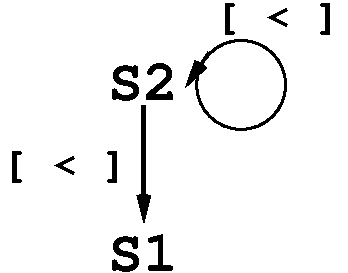
\includegraphics[height=15ex]{img/LoopDistr.pdf}
\end{center}

\noindent and it exhibits two strongly-connected components:
one formed by statement $S_2$ and one formed by statement $S_1$.
Loop distribution results in the following restructured code:
\begin{lstlisting}[mathescape=true]
for (int i = 2; i < N; i++)
  $S_2:$  B[i] = B[i-1] ...
for (int i = 2; i < N; i++)
  $S_1:$  A[i] = B[i-2] ...
\end{lstlisting}
in which, according to the graph order, the loop corresponding to
statement $S_2$ appears before the one corresponding to statement
$S_1$. Note that this does not match the program order of statements
$S_1$ and $S_2$ in the original program. Also note that the first loop
is \emph{not} parallel because the SCC consisting of $S_2$ has a
(dependency) cycle, but the second loop is parallel because the SCC
corresponding to $S_1$ does not have cycles.

If a loop is parallel then it can be straightforwardly distributed
across its statements in program order because:
\begin{itemize}
\item by \cref{Dep-Cycle}, the loop dependency graph has no cycles and
  thereby each statement is a strongly connected component;
\item the program order naturally respects all dependencies.
\end{itemize}

\begin{corollary}[Parallel loop distribution]\label{Par-Loop-Distr}
  A parallel loop can be directly distributed across each one of its
  statements. The resulting loops appear in the same order in which
  their corresponding statements appear in the original loop.
\end{corollary}

\subsection{Array expansion}
\label{sec:array-expansion}

Finally, it remains to demonstrate array expansion, mentioned
in the fourth bullet of \cref{Loop-Distrib}. Assume the slightly
modified code:
\begin{lstlisting}[mathescape=true]
float tmp;
for (int i = 2; i < N; i++) {
  $S_1:$  tmp  = 2 * B[i-2];
  $S_2:$  A[i] = tmp;
  $S_3:$  B[i] = tmp + B[i-1];
}
\end{lstlisting}
Statements $S_1$ and $S_3$ are in a dependency cycle, because
there is a dependency $S_3\to S_1$ with direction \texttt{<} caused
by the write to and the read from array \texttt{B}, and a dependency
$S_1\to S_3$ with direction \texttt{=} caused by \texttt{tmp}.
Statement $S_2$ is not in a dependency cycle, but there is a
dependency $S_1\to S_2$, and hence its distributed loop
should follow the distributed loop containing $S_1$ and $S_3$.
If we do not perform array expansion, the distributed code:

\pagebreak
\begin{lstlisting}[mathescape=true]
float tmp;
for (int i = 2; i < N; i++) {
  $S_1:$  tmp  = 2 * B[i-2];
  $S_3:$  B[i] = tmp + B[i-1];
}
for (int i = 2; i < N; i++) {
  $S_2:$  A[i] = tmp;
}
\end{lstlisting}
\noindent does not respect the semantics of the original program
because the second loop uses the same value of \texttt{tmp}---the one
set by the last iteration of the first loop---while the original loop
writes and then reads a different value of \texttt{tmp} for each
iteration. We fix this by performing array expansion for \texttt{tmp},
which means that we must expand it with an array dimension equal to
the loop count and replace its uses with corresponding indexing
expressions of the expanded array.  This results in the following
\emph{correct} code:

\begin{lstlisting}[mathescape=true]
float tmp[N];
for (int i = 2; i < N; i++) {
  $S_1:$  tmp[j]  = 2 * B[i-2];
  $S_3:$  B[i] = tmp + B[i-1];
}
for (int i = 2; i < N; j++) {
  $S_2:$  A[i] = tmp[j];
}
\end{lstlisting}

Array expansion requires us to normalise the loop first---this means
rewriting the loop such as its index starts from $0$ and increases by
$1$ each iteration. This is why we have not written our example as
\lstinline{do i = 2, N+1}.

\section{Eliminating false dependencies (WAR and WAW)}
\label{sec:false-dep-elim}

Anti and output dependencies are often referred to as \emph{false}
dependencies because they can be eliminated in most cases by copying
or privatisation operations:
\begin{itemize}
\item Cross-iteration anti dependencies (WAR) typically
  correspond to a read from some original element of
  the array---whose value was set before the start of
  the loop execution---followed by an update to that
  element in a later iteration.  As such, this dependency
  can be eliminated by copying (in parallel) the target
  array before the loop and rewriting the offending
  read access inside the loop such that it refers
  to the copy of the array.

\item Cross-iteration output dependencies (WAW) can be
  eliminated by a technique named privatisation (or renaming),
  whenever it can be determined that {\em every read access}
  from a scalar or array location {\em is covered by an
    update} to that scalar or memory location that was
  previously performed {\em in the same iteration}.
  Semantically, privatisation moves the declaration of the
  offending variable inside the loop, because it has been
  already determined that the read/used value was produced
  earlier in the same iteration.

\item Reasoning based on direction vectors is limited to
  relatively simple loop nests; for example it is difficult
  to reason about privatisation by means of direction vectors.
\end  {itemize}

\subsection{Eliminating WAR dependencies by copying}

Consider the simple C code below which rotates an array in the right
dimension by one:

\begin{lstlisting}[mathescape=true]
float tmp = A[0];
for (int i=0; i<N-1; i++) {
    A[i] = A[i+1]; // $S_1$
}
A[N-1] = tmp;
\end{lstlisting}

The loop exhibits a cross-iteration anti dependency (WAR) $S_1\to S_1$
(with direction vector $\texttt{[<]}$), and, as such, it is not safe
to execute it in parallel. However, one can observe that the reads
from \texttt{A} inside the loop correspond to the original elements of
\texttt{A} before the loop, because they are rewritten in a later
iteration.  As such one can perform a copy of \texttt{A} before the
loop, and replace the read access inside the loop to operate on the
copy of array \texttt{A}. This preserves the original loop semantics
and results in a parallel loop because the read and write accesses
operate on different arrays, hence a dependency cannot occur. For
example, using OpenMP:

\begin{lstlisting}[mathescape=true]
float Acopy[N];
#pragma omp parallel for
for (int i=0; i<N; i++) {
    Acopy[i] = A[i];
}
tmp = A[0];
#pragma omp parallel for
for (int i=0; i<N-1; i++) {
    A[i] = Acopy[i+1];
}
A[N-1] = tmp;
\end{lstlisting}

Note that in a real program, we would allocate the \texttt{Acopy}
array with \texttt{malloc()} rather than creating a potentially very
large stack allocation.

\subsection{Eliminating WAW dependencies by privatisation}

Consider the contrived and ugly looking C code below:

\begin{lstlisting}[mathescape=true]
int A[M];
for (int i=0; i<N; i++){
  for (int j=0, j<M; j++) { // writes slice A[0:M-1]
    A[j] = (4*i+4*j) % M;   // $S_1$
  }
  for (int k=0; k<N; k++) { // reads A[j] where j$\in${0,$\ldots$M-1}
                            // because % denotes modulus op
    X[i][k] = X[i][k-1] * A[ A[(2*i+k)%M] % M];      // $S_2$
  }
}
\end{lstlisting}

Analysing the cross-iteration dependencies of the outer loop,
one can observe that there are frequent output dependencies
$S_1\to S_1$ of all directions (\texttt{*}), because, in
essence, all elements of \texttt{A} at indices $0\ldots M-1$
are (over)written in each iteration of the outer loop.
This also causes frequent cross-iteration WAR and RAW
dependencies between $S_1$ and $S_2$ of all directions
\texttt{*} because $S_2$ reads some of the values of
\texttt{A} which are written in $S_1$. The read access
is also statically unanalysable because the index
into \texttt{A} depends on a value of \texttt{A} (i.e.,
it is an indirect-array access \texttt{A[ A[...] ]}).

It would thus seem that this is a hopeless case and parallel
execution is a pipe dream. Not so! Actually the rationale
of how to transform the outer loop into a parallel one
is quite simple.  One may observe that each iteration of
the outer loop writes the same indices of \texttt{A}, namely
the ones belonging to the closed integral interval
\texttt{[0,M-1]}.   One may also observe that $S_2$ reads
from \texttt{A} elements whose indices necessarily belong to
\texttt{[0,M-1]}---due to the two modulus-\texttt{M} operations.
As such, one may conclude that any value
read in $S_2$ must have been produced in the same iteration
of the outer loop (in the inner loop enclosing $S_1$).

It follows that it is safe to rewrite the loop in the
following way:
\begin{enumerate}
\item Declare a new variable \texttt{A'} of the same dimensions as
  \texttt{A} just inside the outer loop (or equivalently perform array
  expansion of array \texttt{A'} with a new outer dimension of size
  \texttt{N}).
\item Replace all the uses of \texttt{A} in the outer loop by uses of
  \texttt{A'}.  The resulting loop is safe to execute in parallel
  because there can be no dependencies on \texttt{A'} since each
  iteration uses a different array \texttt{A'}.
\item As a last step, after the parallel execution of the loop
  terminates, one must copy (in parallel) the elements produced by the
  last iteration of the outer loop (i.e., \texttt{A'[0,$\ldots$][M-1]}
  back to \texttt{A}.
\end{enumerate}

The parallel OpenMP code that implements these steps is
presented below:

\begin{lstlisting}[mathescape=true]
int A[M];
#pragma omp for lastprivate(A)
for (int i=0; i<N; i++) {
    for(int j=0, j<M; j++) {
        A[j] = (4*i+4*j) % M;
    }
    for(int k=0; k<N; k++) {
        X[i][k]=X[i][k-1] * A[ A[(2*i+k) % M] % M];
    }
}
\end{lstlisting}

Declaring array \texttt{A} as private (by using the clause
\texttt{private(A)}) would result in semantically performing steps (1)
and (2) above. Using the \texttt{lastprivate(A)} clause instructs the
OpenMP compiler to also perform step (3)---to copy back the
privately-maintained result of \texttt{A} of the last executing
iteration into the globally-declared array \texttt{A}.

Please also note that the OpenMP execution will not allocate
a new \texttt{A'} for each iteration of the outer loop---this is
actually equivalent to performing array expansion which is also
applicable here---but instead it will {\em allocate a copy of
  \texttt{A} for each active thread}, thus significantly reducing
the memory footprint and/or the number of (de)allocations.

Privatisation can be applied whenever one can prove that every read
access in an iteration is covered by a previously-performed write
access in the same iteration.  Privatisation can be implemented by
performing either array expansion or moving the declaration of the
target variable from outside to inside the loop. However, it saves
memory to allocate the private copy per active thread rather than per
iteration, which is what OpenMP is doing.

\section{Loop stripmining, block and register tiling}
\label{sec:strip-tiling}

This section discusses several simple transformations that are going
to be combined in various ways to optimise locality of reference (both
temporal and spatial locality).

\textbf{\em Stripmining} refers to the following transformation,
which is always safe to apply:
\begin{lstlisting}[mathescape=true]
for(int i = 0; i<N; i++) {      for(int ii = 0; ii<N; ii+=T){
  iteration body            $\Rightarrow$    for(int i=ii, i<min(ii+T,N); i++)
}                                     iteration body
                                } }
\end{lstlisting}
In essence, a normalized loop is split into a perfect nest of two
loops, in which the first loop goes with stride \texttt{T}, and
the second one goes with stride \texttt{1}. Please notice that the
resulting loop nest executes the same number of statements and
in the same order as the original loop.

\textbf{\em Block tiling} refers to the transformation that
stripmines several consecutive innermost loops in a
perfect loop nest---named $l_{k+1}\ldots l_{k+n}$---and then
interchanges inwards the resulting loops of stride $1$.
The transformation is valid/safe if in the original program
it is safe to interchange any of the loops
$l_{k+i},~i\in\{1,\ldots,n-1\}$ in the innermost position.
For example, the code below demonstrates block tiling a perfect
loop nest of depth two:
\begin{lstlisting}[mathescape=true]
for(i = 0; i<N; i++) {      for(ii=0; ii<N; ii+=T1) {
  for(j = 0; j<M; j++) {      for(jj=0; jj<M; jj+=T2) {
    iteration body       $\Rightarrow$     for(i=ii; i<min(ii+T1,N); i++) {
  }                               for(j=jj; j<min(jj+T2,M); j++) {
}                                   iteration body
                            } } } }
\end{lstlisting}

\textbf{\em Unroll and jam} refers to the transformation that partially
unrolls one or more of the outer loops in a perfect nest and then
fuses (``jams'') the resulting loops. Equivalently, one can stripmine
an outer loop, then interchange (distribute) it in the innermost
position, then completely unroll it. The transformation is aimed at
decreasing the number of memory loads and stores by storing to and
reusing values from registers, and thus it is applied when the
original loop nest contains data references that allow for temporal
reuse---e.g., their indexes are invariant to some of the loops
in the nest.
Due to this, it is also known as ``{\em register tiling}''.
We demonstrate the transformation on the matrix-matrix
multiplication code below:
\begin{lstlisting}[mathescape=true]
for(i=0; i<N; i++) {
  for(j=0; j<M; j++) {
    float c;
    c = 0.0;
    for(k=0; k<N; k++) {
      c += A[i][k] * B[k][j];
    }
    C[i][j] = c;
  }
}
\end{lstlisting}

The plan is to stripmine the loop of index \texttt{j} by a tile of
size $2$, and to interchange it to the innermost position, while
performing the necessary loop distribution and array expansion:
\begin{lstlisting}[mathescape=true]
for(i=0; i<N; i++) {
  for(jj=0; jj<M; jj+=2) {
    float cs[2];
    for(j=jj; j<min(jj+2,M); j++) {
        cs[j-jj] = 0.0;
    }
    for(k=0; k<N; k++) {
      for(j=jj; j<min(jj+2,M); j++) {
        cs[j-jj] += A[i][k] * B[k][j];
    } }
    for(j=jj; j<min(jj+2,M); j++) {
        C[i][j] = cs[j-jj];
    }
} }
\end{lstlisting}
One can observe that the access \texttt{A[i][k]} is invariant to its
immediately contained loop of index \texttt{j} and thus it can be hoisted
outside it and saved into a register. Then the loops of index \texttt{j}
can be unrolled, and array \texttt{cs} can be scalarized as well:
\begin{lstlisting}[mathescape=true]
for(i=0; i<N; i++) {
  for(jj=0; jj<M; jj+=2) {
    float c1, c2;
    if (jj   < M) c1 = 0.0;
    if (jj+1 < M) c2 = 0.0;
    for(k=0; k<N; k++) {
      float a;
      a = A[i,k];
      if (jj   < M) c1 += a * B[k][jj  ];
      if (jj+1 < M) c2 += a * B[k][jj+1];
    }
    if (jj   < M) C[i][jj  ] = c1;
    if (jj+1 < M) C[i][jj+1] = c2;
} }
\end{lstlisting}
In the resulted code, the accesses to the elements of \texttt{A} have
been halved.   We can similarly apply unroll and jam for the loop
of index \texttt{i} with a tile size equal to \texttt{3}. This will cut down
the accesses to \texttt{B} by a factor of $3$. The resulted code
is shown in \cref{fig-unroll-jam}.

\begin{figure}
\begin{lstlisting}[mathescape=true]
for(ii=0; ii<N; ii+=3) {
  for(jj=0; jj<M; jj+=2) {

    float c11, c12, c21, c22, c31, c32;

    if (ii   < N && jj   < M) c11 = 0.0;
    if (ii+1 < N && jj   < M) c21 = 0.0;
    if (ii+2 < N && jj   < M) c31 = 0.0;
    if (ii   < N && jj+1 < M) c12 = 0.0;
    if (ii+1 < N && jj+1 < M) c22 = 0.0;
    if (ii+2 < N && jj+1 < M) c32 = 0.0;

    for(k=0; k<N; k++) {

      float a1, a2, a3, b1, b2;

      if (ii   < N) a1 = A[ii  ][k];
      if (ii+1 < N) a2 = A[ii+1][k];
      if (ii+2 < N) a3 = A[ii+2][k];
      if (jj   < M) b1 = B[k   ][jj];
      if (jj+1 < M) b2 = B[k   ][jj+1];

      if (ii   < N && jj   < M) c11 += a1 * b1;
      if (ii+1 < N && jj   < M) c21 += a2 * b1;
      if (ii+2 < N && jj   < M) c31 += a3 * b1;
      if (ii   < N && jj+1 < M) c12 += a1 * b2;
      if (ii+1 < N && jj+1 < M) c22 += a2 * b2;
      if (ii+2 < N && jj+1 < M) c32 += a3 * b2;
    }

    if (ii   < N && jj   < M) C[ii  ][jj  ] = c11;
    if (ii+1 < N && jj   < M) C[ii+1][jj  ] = c21;
    if (ii+2 < N && jj   < M) C[ii+2][jj  ] = c31;
    if (ii   < N && jj+1 < M) C[ii  ][jj+1] = c11;
    if (ii+1 < N && jj+1 < M) C[ii+1][jj+1] = c21;
    if (ii+2 < N && jj+1 < M) C[ii+2][jj+1] = c31;
  }
}
\end{lstlisting}
  \caption{Result of unroll-and-jam applied to matrix-matrix
    multiplication, where the first and second outer loops were tiled
    with sizes $3$ and $2$, respectively. The number of accesses to
    \texttt{A} and \texttt{B} has been reduced by a factor of
    $2\times$ and $3\times$, respectively, at the expense of
    introducing some conditional statements.}
  \label{fig-unroll-jam}
\end{figure}

%%% Local Variables:
%%% mode: latex
%%% TeX-master: "notes"
%%% End:


\newpage

\bibliographystyle{plain}
\bibliography{notes}

\end{document}

%%% Local Variables:
%%% mode: latex
%%% TeX-master: t
%%% End:
